% (c)~2014 Claudio Carboncini - claudio.carboncini@gmail.com
% (c)~2014 Dimitrios Vrettos - d.vrettos@gmail.com
\section{Esercizi}
\subsection{Esercizi dei singoli paragrafi}
\subsection*{3.1 - le equazioni di secondo grado in una incognita}

\begin{esercizio}[\Ast]
 \label{ese:3.1}
Risolvi le seguenti equazioni di secondo grado pure.
\begin{multicols}{3}
 \begin{enumeratea}
 \item~$x^{2}-1 = 0$;
 \item~$x^{2}=\frac{49}{25}$;
 \item~$2x^{2} - 32 = 0$;
 \item~$x^{2}-25=0$;
 \item~$16 x^{2}=1$;
 \item~$3x^{2}+3=0$;
 \item~$x^{2}-9=0$;
 \item~$25=9 x^{2}$;
 \item~$x^{2} - 3 = 0$;
 \item~$x^{2} + 36 = 0$;
 \item~$4 - x^{2} = 0$;
 \item~$x^{2} + 4 = 0$.
 \end{enumeratea}
 \end{multicols}
\end{esercizio}

\begin{esercizio}[\Ast]
\label{ese:3.2}
Risolvi le seguenti equazioni di secondo grado pure.
\begin{multicols}{3}
 \begin{enumeratea}
 \item~$x^{2} = 49$;
 \item~$4 - 9 x^{2} = 0$;
 \item~$5 x^{2} - 3 = 0$;
 \item~$4 x^{2} - 9 = 0$;
 \item~$9 x^{2} - 25 = 0$;
 \item~$6 x^{2} = 0$;
 \item~$2 x^{2} - 1 = 0$;
 \item~$4 x^{2} + 16 = 0$;
 \item~$1 + x^{2} = 50$;
 \item~$3 x^{2} - 1 = 0$;
 \item~$27 x^{2} - 3 = 0$;
 \item~$7 x^{2} = 28$.
 \end{enumeratea}
 \end{multicols}
\end{esercizio}

\begin{esercizio}[\Ast]
 \label{ese:3.3}
Risolvi le seguenti equazioni di secondo grado pure.
\begin{multicols}{3}
 \begin{enumeratea}
 \item~$4 x^{2} - 4 = 0$;
 \item~$5 x^{2} - 125 = 0$;
 \item~$0,04 x^{2} = 1$;
 \item~$x^{2} - 0,01 = 0$;
 \item~$0,5 x^{2} - 4,5 = 0$;
 \item~$0,09 x^{2} = 0,01$;
 \item~$\frac{1}{2} x^{2} - 2 = 0$;
 \item~$x^{2} - \frac{9}{4} = 0$;
 \item~$x^{2} - \frac{1}{6} = 0$;
 \item~$121 x^{2} - \frac{1}{169} = 0$;
 \item~$x^{2} + \frac{9}{4} = 0$;
 \item~$4 \left(x^{2}-\frac{3}{4}\right)= 13$.
 \end{enumeratea}
 \end{multicols}
\end{esercizio}

\begin{esercizio}[\Ast]
 \label{ese:3.4}
Risolvi le seguenti equazioni di secondo grado pure.
\begin{multicols}{2}
 \begin{enumeratea}
 \item~$x^{2} - \sqrt{3} = 0$;
 \item~$- 9 x^{2} = - 1$;
 \item~$4 x^{2} = - 9$;
 \item~$x^{2} + 6 = 42$;
 \item~$5 - 125 x^{2} = 0$;
 \item~$18 - x^{2} = 0$;
 \item~$(x + 3)^{2} = 6 x + 34$;
 \item~$(x + 1)^{2} = 25$;
 \item~$(x - \sqrt{3}) (x + \sqrt{3}) = 13$;
 \item~$(x + \sqrt{2})^{2} = 2 \sqrt{2} x$;
 \item~$(x - 2)^{2} + (1 - x)^{2} = 1 - 6x$;
 \item~$(\sqrt{2} x - \sqrt{3}) (\sqrt{2} x + \sqrt{3}) = 0$.
 \end{enumeratea}
 \end{multicols}
\end{esercizio}

\begin{esercizio}[\Ast]
\label{ese:3.5}
Risolvi le seguenti equazioni di secondo grado spurie.
\begin{multicols}{3}
 \begin{enumeratea}
 \item~$x^{2} - 3 x = 0$;
 \item~$3 x^{2} - 2 x = 0$;
 \item~$7 x^{2} + 2 x = 0$;
 \item~$x^{2} + 2 x = 0$;
 \item~$x^{2} + 5 x = 0$;
 \item~$x^{2} - x = 0$.
 \end{enumeratea}
 \end{multicols}
\end{esercizio}

\begin{esercizio}[\Ast]
\label{ese:3.6}
Risolvi le seguenti equazioni di secondo grado spurie.
\begin{multicols}{3}
 \begin{enumeratea}
 \item~$18 x^{2} - 36 x = 0$;
 \item~$2x^{2} + 6x = 0$;
 \item~$1000 x - 2000 x^{2} = 0$;
 \item~$9x^{2} + 16x = 0$;
 \item~$6 x^{2} = 5 x$;
 \item~$5x = 25x^{2}$.
 \end{enumeratea}
 \end{multicols}
\end{esercizio}
\newpage
\begin{esercizio}[\Ast]
 \label{ese:3.7}
Risolvi le seguenti equazioni di secondo grado spurie.
\begin{multicols}{3}
 \begin{enumeratea}
 \item~$3 x^{2} - 2 x = 4 x$;
 \item~$81x^{2} = 9x$;
 \item~$0,1 x^{2} - 0,5 x = 0$;
 \item~$7x^{2} - 2x = 0$;
 \item~$0,5 x^{2} + 0,1 x = 0$;
 \item~$x^{2} + \frac{1}{2} x = 0$.
 \end{enumeratea}
 \end{multicols}
\end{esercizio}

\begin{esercizio}[\Ast]
 \label{ese:3.8}
Risolvi le seguenti equazioni di secondo grado spurie.
\begin{multicols}{3}
 \begin{enumeratea}
 \item~$\frac{1}{2} x - \frac{1}{4} x^{2} = 0$;
 \item~$\sqrt{2} x^{2} + \sqrt{3} x = 0$;
 \item~$x^{2} + \sqrt{2} x = 0$;
 \item~$- 2x^{2} + 4x = 0$;
 \item~$5 \sqrt{2} x^{2} - 2 \sqrt{2} x = 0$;
 \item~$\frac{1}{6} x^{2} + \frac{1}{4} x = 0$.
 \end{enumeratea}
 \end{multicols}
\end{esercizio}

\begin{esercizio}[\Ast]
 \label{ese:3.9}
Risolvi le seguenti equazioni di secondo grado spurie.
\begin{multicols}{3}
 \begin{enumeratea}
 \item~$3x^{2} - \frac{4}{3} x = 0$;
 \item~$(x - 2)^{2} = 4$;
 \item~$(x + 1)^{2} = 1$;
 \item~$(x + \sqrt{2})^{2} = 2$;
 \item~$77 x - 11 x^{2} = 0$;
 \item~$\frac{3}{4} x^{2} - \frac{3}{2} x = 0$.
 \end{enumeratea}
 \end{multicols}
\end{esercizio}

\begin{esercizio}[\Ast]
 \label{ese:3.10}
Risolvi le seguenti equazioni di secondo grado spurie.
\begin{multicols}{2}
 \begin{enumeratea}
 \item~$\frac{11}{3} x^{2} = - 2 x$;
 \item~$\frac{1}{2} ( x - 2 )^{2} - x = 2$;
 \item~$(x - 1) (x + 3) = 3 x^{2} - 3$;
 \item~$(3 x - 2)^{2} - 4 = 6 x^{2}$.
 \end{enumeratea}
 \end{multicols}
\end{esercizio}

\begin{esercizio}[\Ast]
 \label{ese:3.11}
Risolvi le seguenti equazioni di secondo grado spurie.
 \begin{enumeratea}
 \item~$(x - 2)^{2} + (1 - x)^{2} = 5$;
 \item~$(x - 2)^{3} - 4 (2 x - 1) = (x + 2) \left(x^{2} - 2 x + 4\right) - 12$;
 \item~$(\sqrt{2} + x)^{3} - (\sqrt{3} + x)^{3} = 2 \sqrt{2} - 3\sqrt{3}$;
 \item~$(\sqrt{2} x - \sqrt{3}) (\sqrt{2} x + \sqrt{3}) + (\sqrt{3} x + \sqrt{3})^{2} + (x - 1)^{2} = 1$;
 \item~$\left(x^{2} + \sqrt{2} \right) (\sqrt{3} - 1) + (2 x +\sqrt{3}) (\sqrt{2} - 1) - \sqrt{2} + \sqrt{3} = 0$.
 \end{enumeratea}
\end{esercizio}

\subsection*{3.2 - Risoluzione di un'equazione completa}
\begin{esercizio}[\Ast]
 \label{ese:3.12}
Risolvi le seguenti equazioni di secondo grado complete.
\begin{multicols}{2}
 \begin{enumeratea}
 \item~$x^{2}-5 x + 6=0$;
 \item~$x^{2} + x-20=0$;
 \item~$2 x^{2}-6 x-6=0$;
 \item~$x^{2}-3 x + 6=0$.
 \end{enumeratea}
 \end{multicols}
\end{esercizio}

\begin{esercizio}
 \label{ese:3.13}[\Ast]
Risolvi le seguenti equazioni di secondo grado complete.
\begin{multicols}{2}
 \begin{enumeratea}
 \item~$- x^{2} + x + 42=0$;
 \item~$- x^{2} + 10 x-25=0$;
 \item~$- 2 x^{2} + 7 x-5=0$;
 \item~$3 x^{2} + 2 x-1=0$.
 \end{enumeratea}
 \end{multicols}
\end{esercizio}

\begin{esercizio}[\Ast]
 \label{ese:3.14}
Risolvi le seguenti equazioni di secondo grado complete.
\begin{multicols}{2}
 \begin{enumeratea}
 \item~$2 x^{2}-\sqrt{5} x-1 = 0$;
 \item~$x^{2}-2 \sqrt{3} x-4=0$;
 \item~$x^{2}-3 x-2=0$;
 \item~$2 x^{2}-\sqrt{5} x-1=0$.
 \end{enumeratea}
 \end{multicols}
\end{esercizio}
\newpage
\begin{esercizio}[\Ast]
 \label{ese:3.15}
Risolvi le seguenti equazioni di secondo grado complete.
\begin{multicols}{2}
 \begin{enumeratea}
 \item~$- \frac{4}{3} x^{2}-x + \frac{3}{2}=0$;
 \item~$- \frac{4}{5} x^{2} + \frac{1}{2} x-\frac{1}{20}=0$;
 \item~$- x^{2} + 4 x-7=0$;
 \item~$x^{2}-\sqrt{5} x-\sqrt{5}=0$.
 \end{enumeratea}
 \end{multicols}
\end{esercizio}

\begin{esercizio}[\Ast]
 \label{ese:3.16}
Risolvi le seguenti equazioni di secondo grado complete.
\begin{multicols}{2}
 \begin{enumeratea}
 \item~$x^{2}-5 x + 3 = 0$;
 \item~$x^{2}-4 x + 9 = 0$;
 \item~$x^{2}-4 x-9 = 0$;
 \item~$x^{2} + 6 x-2 = 0$.
 \end{enumeratea}
 \end{multicols}
\end{esercizio}

\begin{esercizio}[\Ast]
 \label{ese:3.17}
Risolvi le seguenti equazioni di secondo grado complete.
\begin{multicols}{2}
 \begin{enumeratea}
 \item~$x^{2}-3 x-\frac{5}{2} = 0$;
 \item~$2 x^{2}-3 x + 1 = 0$;
 \item~$\frac{4}{3} x^{2}-\frac{1}{3} x-1 = 0$;
 \item~$3 x^{2} + x-2 = 0$.
 \end{enumeratea}
 \end{multicols}
\end{esercizio}

\begin{esercizio}[\Ast]
 \label{ese:3.18}
Risolvi le seguenti equazioni di secondo grado complete.
\begin{multicols}{2}
 \begin{enumeratea}
 \item~$3 x^{2}-\frac{2}{3} x-1 = 0$;
 \item~$\sqrt{2} x^{2}-x-3 \sqrt{2} = 0$;
 \item~$x^{2}-(\sqrt{2} + \sqrt{3}) x + \sqrt{6} = 0$;
 \item~$x^{2} + (\sqrt{2}-\sqrt{3}) x-\sqrt{6} = 0$.
 \end{enumeratea}
 \end{multicols}
\end{esercizio}

\begin{esercizio}[\Ast]
 \label{ese:3.19}
Risolvi le seguenti equazioni di secondo grado complete.
\begin{multicols}{2}
 \begin{enumeratea}
 \item~$(3 x + 1)^{2}-(2 x + 2)^{2} = 0$;
 \item~$(x + 5)^{2} = 5 (4 x + 5)$;
 \item~$(x-2) (3-2 x) = x-2$;
 \item~$(x + 200)^{2} + x + 200 = 2$;
 \item~$(x^{2} + x + 1) (x^{2}-x-1) = (x^{2}-1)^{2}$.
 \end{enumeratea}
 \end{multicols}
\end{esercizio}

\begin{esercizio}[\Ast]
\label{ese:3.20}
Risolvi, applicando quando possibile la formula ridotta o ridottissima.
\begin{multicols}{2}
 \begin{enumeratea}
 \item~$3 x^{2}-2 x-2 = 0$;
 \item~$x^{2} + 6 x-3 = 0$;
 \item~$4 x^{2}-8 x + 3 = 0$;
 \item~$7 x^{2}-2 x-5 = 0$.
 \end{enumeratea}
 \end{multicols}
\end{esercizio}

\begin{esercizio}[\Ast]
\label{ese:3.21}
Risolvi, applicando quando possibile la formula ridotta o ridottissima.
\begin{multicols}{2}
 \begin{enumeratea}
 \item~$40 x^{2} + 80 x-30 = 0$;
 \item~$5 x^{2}-4 x + 1 = 0$;
 \item~$5 x^{2}-4 x-9 = 0$;
 \item~$\frac{3}{2} x^{2} + 2 x-\frac{3}{4} = 0$.
 \end{enumeratea}
 \end{multicols}
\end{esercizio}

\begin{esercizio}[\Ast]
 \label{ese:3.22}
Risolvi, applicando quando possibile la formula ridotta o ridottissima.
\begin{multicols}{2}
 \begin{enumeratea}
 \item~$6 x^{2}-4 x-2 = 0$;
 \item~$90 x^{2}-180 x-270 = 0$;
 \item~$\frac{3}{2} x^{2}-4 x + 2 = 0$;
 \item~$\frac{4}{3} x^{2}-6 x + 6 = 0$.
 \end{enumeratea}
 \end{multicols}
\end{esercizio}

\begin{esercizio}[\Ast]
\label{ese:3.23}
Risolvi, applicando quando possibile la formula ridotta o ridottissima.
\begin{multicols}{2}
 \begin{enumeratea}
 \item~$x^{2}-6 x + 1 = 0$;
 \item~$3 x^{2}-12 x-3 = 0$;
 \item~$7 x^{2}-6 x + 8 = 0$;
 \item~$3 x^{2}-18 x + 27 = 0$.
 \end{enumeratea}
 \end{multicols}
\end{esercizio}
\newpage
\begin{esercizio}[\Ast]
\label{ese:3.24}
Risolvi, applicando quando possibile la formula ridotta o ridottissima.
\begin{multicols}{2}
 \begin{enumeratea}
 \item~$9 x^{2} + 12 x + 1 = 0$;
 \item~$9 x^{2}-12 x + 4 = 0$;
 \item~$4 x^{2}-32 x + 16 = 0$;
 \item~$3 x^{2} + 10 x + 20 = 0$.
 \end{enumeratea}
 \end{multicols}
\end{esercizio}

\subsection*{Altri esercizi sulle equazioni di 2° grado}

\begin{esercizio}[\Ast]
\label{ese:3.25}
Risolvi le seguenti equazioni di secondo grado.
\begin{multicols}{2}
 \begin{enumeratea}
 \item~$(3 x + 1) \left(\frac{5}{2} + x \right) = 2 x-1$;
 \item~$(3 x-2)^{2} + (5 x-1)^{2} = (3 x-2) (5 x-1)$;
 \item~$3 x-x^{2} = x^{2} + 3 (x-2)$;
 \item~$2 (x-1) (x + 1) = 2$.
 \end{enumeratea}
 \end{multicols}
\end{esercizio}

\begin{esercizio}[\Ast]
 \label{ese:3.26}
Risolvi le seguenti equazioni di secondo grado.
\begin{multicols}{2}
 \begin{enumeratea}
 \item~$(2 x-1) (4-x)-11 x = (1-x)^{2}$;
 \item~$2x^{2} = x + x^{2}-(x + \sqrt{x}) (x-\sqrt{x})$;
 \item~$(x-3)^{2} = 9-6 x$;
 \item~$(x-2)^{3}-1 = x^{3} + 12 x-11$.
 \end{enumeratea}
 \end{multicols}
\end{esercizio}

\begin{esercizio}[\Ast]
 \label{ese:3.27}
Risolvi le seguenti equazioni di secondo grado.
\begin{multicols}{2}
 \begin{enumeratea}
 \item~$\frac{3 x-2}{2} = x^{2}-2$;
 \item~$(2 x-3) (2 x + 3) = 27$;
 \item~$\frac{x-3}{2}-\frac{x^{2} + 2}{3} = 1 + x$;
 \item~$\frac{x-2}{3}-(3 x + 3)^{2} = x$.
 \end{enumeratea}
 \end{multicols}
\end{esercizio}

\begin{esercizio}[\Ast]
 \label{ese:3.28}
Risolvi le seguenti equazioni di secondo grado.
\begin{multicols}{2}
 \begin{enumeratea}
 \item~$(x-2)^{3}-x^{3} = x^{2}-4$;
 \item~$x (1-5 x) = [ 3-(2 + 5 x) ] x-(x^{2}-1)$;
 \item~$(x + 1)^{3}-(x + 2)^{2} = \frac{2 x^{3}-1}{2}$;
 \item~$\frac{(x-1)^{2}}{2}-\frac{2 x-5}{3} =-\frac{5}{3} x$.
 \end{enumeratea}
 \end{multicols}
\end{esercizio}

\begin{esercizio}[\Ast]
 \label{ese:3.29}
Risolvi le seguenti equazioni di secondo grado.
\begin{multicols}{2}
 \begin{enumeratea}
 \item~$(x + 2)^{3} + 4 x^{2} = (x-2)^{3} + 16$;
 \item~$(2-x)^{3}-(2-x)^{2} = \frac{3-4 x^{3}}{4}$;
 \item~$3 \left(x + \sqrt{2} \right)^{2}-18 \left(x + \sqrt{2}\right) + 27 = 0$;
 \item~$(4-3 x)^{3} + 27 x^{3} = 64 + 24 x$.
 \end{enumeratea}
 \end{multicols}
\end{esercizio}

\begin{esercizio}[\Ast]
 \label{ese:3.30}
Risolvi le seguenti equazioni di secondo grado.
 \begin{enumeratea}
 \item~$\left(\frac{x-1}{3}-\frac{x}{6} \right)^{2} = (x + 1)^{2}$;
 \item~$(\sqrt{3} x + 1)^{2} + (\sqrt{3} x-1)^{2}-3 (\sqrt{3} b x + 1) (\sqrt{3} x-1) = 0$;
 \item~$\frac{(2 x + 1) (x-2)}{3} + \frac{(x + \sqrt{5}) (x -\sqrt{5})}{2} = \frac{(x-1)^{2}}{6}$;
 \item~$\left(\frac{1}{2} x + 1 \right)^{3} = \left(\frac{1}{2} x-1\right) \left(\frac{1}{2} x + 1 \right)^{2}$.
 \end{enumeratea}
\end{esercizio}


\begin{esercizio}[\Ast]
 \label{ese:3.31}
Risolvi le seguenti equazioni di secondo grado.
 \begin{enumeratea}
 \item~$\frac{(3 x-1)^{2}}{3}-\frac{(1-2 x)^{2}}{5} + \frac{3 x (x-1)}{5} + \frac{(1 + x)^{2}}{3} = 0$;
 \item~$\frac{1}{\sqrt{10}} x^{2} + 1 = \left(\frac{1}{\sqrt{2}} +\frac{1}{\sqrt{5}} \right) x$;
 \item~$(3 x-1)^{2} + (2 x + 1)^{2} = (3 x-1) (2 x + 1)$;
 \item~$(x + 1)^{4}-(x + 1)^{3} = x^{3} (x + 4)-x (x + 1)^{2} + 3 x$.
 \end{enumeratea}
\end{esercizio}
\newpage
\begin{esercizio}[\Ast]
 \label{ese:3.32}
Risolvi le seguenti equazioni di secondo grado.
 \begin{enumeratea}
 \item~$\left(\frac{1}{2} x^{2} + 1 \right)^{3} + \frac{1}{6} x^{3} = \left(\frac{1}{2} x^{2}-1 \right)^{3} + \frac{1}{6} (x + 1)^{3} + \frac{3}{2} x^{4}$;
 \item~$\frac{x-2}{2} \cdot \frac{x + 2}{3} + \frac{1}{3} \left[\frac{1}{2}-\left(x + \frac{1}{2} \right) \right] + 4 \left(x -\frac{1}{2} \right) \left(x + \frac{1}{2} \right) + \frac{5}{3} = 0$;
 \item~$(2-3 x)^{2}-1 = 8 (1-2 x) + (2 x + 1)^{2}-1$;
 \item~$x^{2} + \left(\sqrt{3}-\sqrt{2} \right) x-\sqrt{6} = 0$.
 \end{enumeratea}
\end{esercizio}

\begin{esercizio}[\Ast]
 \label{ese:3.33}
Risolvi le seguenti equazioni di secondo grado.
 \begin{enumeratea}
 \item~$\frac{2 \sqrt{3} x + 1}{\sqrt{2}}-\left(x-\sqrt{3} \right)^{2} = \frac{1-3 \sqrt{2} x}{\sqrt{2}} + \sqrt{3} x \left(\sqrt{2}+ 2 \right)$;
 \item~$\sqrt{3} (2 x-30)^{2}-2 \sqrt{27} (60-4 x) = 0$;
 \item~$\left(2 x + \frac{1}{2} \right)^{2}-\frac{1}{2} \left(\frac{1}{2} x-1 \right)^{2} + \left(x-\frac{1}{2} \right) \left(x + \frac{1}{2} \right) = 0$;
 \item~$\frac{x^{2}-16}{9} + \frac{(x-1)^{2}}{3} = \frac{x (x -2)}{9} + \left(x-\frac{5}{2} \right) \left(x + \frac{1}{3}\right)$.
 \end{enumeratea}
\end{esercizio}

 \begin{esercizio}[\Ast]
\label{ese:3.34}
Risolvi le seguenti equazioni di secondo grado.
 \begin{enumeratea}
 \item~$\frac{(x-1) (x + 2)}{2} + \frac{(x + 2) (x-3)}{3} =\frac{(x-3) (x + 4)}{6}$;
 \item~$\left(2 x-\frac{1}{2} \right)^{2} + \left(\frac{x-1}{2} -\frac{x}{3} \right) x =-x^{2} + \frac{2}{3} \left(x-\frac{1}{2}\right) x-\frac{1}{2} x + \frac{1}{9}$;
 \item~$\frac{1}{4} (2 x-1)^{2}-\frac{1}{3} (x-1)^{2} +\frac{(x-2) (x + 2)}{2}-\frac{1}{6} x + \frac{1}{6} = 0$;
 \item~$\frac{1}{2} (2 x-1) (x + 1) + \frac{1}{3} \left(x^{2}-5\right) + 2 x (x-1) (x + 1) = 2 (x + 2)^{3}-(2 x-1)^{2}$.
 \end{enumeratea}
\end{esercizio}

\begin{esercizio}[\Ast]
\label{ese:3.35}
Risolvi le seguenti equazioni di secondo grado.
 \begin{enumeratea}
 \item~$\frac{3 x-1}{\sqrt{5}-\sqrt{3}} + \frac{\left(x-\sqrt{3}\right) \left(x + \sqrt{3} \right)}{\sqrt{3}}-\frac{\left(x -\sqrt{3} \right)^{2}}{\sqrt{3}} = \frac{x^{2}}{\sqrt{5}-\sqrt{3}} + 2 x-2 \sqrt{3}$;
 \item~$\left(x + \frac{1}{2} \right)^{2}-\frac{3 x^{2}-7 x + 2}{2} - \frac{x}{4} + \frac{5 x-13}{2} = \frac{2}{3} x (1-x) +\frac{73}{12} x-\frac{15}{12}$;
 \item~$\frac{(x^{2} + 2 x + 1)^{2}}{4} + \frac{(x + 1)^{2}}{2}+ \frac{(x^{4}-1)}{8}-(2 x^{2}-2 x + 1)^{2} + 9 x^{3}\left(\frac{3}{8} x-1 \right) + \frac{1}{4} x^{2} (x^{2} + 20)= 0$.
 \end{enumeratea}
\end{esercizio}

\begin{esercizio}[\Ast]
 \label{ese:3.36}
Risolvi le seguenti equazioni con opportune sostituzioni.
\begin{multicols}{2}
\begin{enumeratea}
\item $(4x + 3)^{2} = 25$;
\item $(x-5)^{2} + 9 = 0$;
\item $(3x-1)^{2}-36 = 0$;
\item $4 (2x + 1)^{2} = 36$.
\end{enumeratea}
\end{multicols}
\end{esercizio}

\begin{esercizio}[\Ast]
\label{ese:3.37}
Risolvi le seguenti equazioni con opportune sostituzioni.
\begin{multicols}{2}
\begin{enumeratea}
\item $(3x-5)^{2}-49 = 0$;
\item $3 (2x + 5)^{2}-4 (2x + 5) = 0$;
\item $(3 \cdot 10^{3} x-10)^{2}-5 (3 \cdot 10^{3} x-10) = -6$;
\item $(x-1)^{2}-(\sqrt{3} + \sqrt{5}) (x-1) + \sqrt{15} =0$.
\end{enumeratea}
\end{multicols}
\end{esercizio}

\begin{esercizio}[\Ast]
\label{ese:3.38}
Risolvi le seguenti equazioni con opportune sostituzioni.
\begin{multicols}{2}
\begin{enumeratea}
\item $3 (1-2x)^{2}-2 (1-2x)-1 = 0$;
\item $\frac{4}{3} (x-2)^{2}-6 (x-2) + 6 = 0$;
\item $\frac{1}{2} \left(x-\frac{1}{2} \right)^{2}-2 \left(x -\frac{1}{2} \right) = 0$;
\item $2 (x^{2}-1)^{2} + 3 (x^{2}-1)-5 = 0$;
\item $3 (34 x-47)^{2}-2 (34 x-47) = 1$.
\end{enumeratea}
\end{multicols}
\end{esercizio}
\newpage
\subsection*{3.3 - Discussione e risoluzione di equazioni numeriche frazionarie}

\begin{esercizio}[\Ast]
\label{ese:3.39}
Determina l'Insieme Soluzione delle seguenti equazioni fratte.
\begin{multicols}{2}
\begin{enumeratea}
\item $\frac{3}{x}-2 = x$;
\item $\frac{4-3 x}{x}=\frac{3-2 x}{x^{2}}$;
\item $\frac{1}{x} = \frac{1}{x + 1}-1$;
\item $\frac{x}{2} = \frac{x + 2}{x-2} + 1$.
\end{enumeratea}
\end{multicols}
\end{esercizio}

\begin{esercizio}[\Ast]
\label{ese:3.40}
Determina l'Insieme Soluzione delle seguenti equazioni fratte.
\begin{multicols}{2}
\begin{enumeratea}
\item $\frac{3}{x-1}-\frac{1}{x} + \frac{1}{2} = 0$;
\item $\frac{3 x}{x^{2}-9} + \frac{x}{2 x-6}=1$;
\item $\frac{x + 9}{x-3}=2-\frac{x-3}{x + 9}$;
\item $\frac{x}{x + 1} = \frac{4}{x + 2}$.
\end{enumeratea}
\end{multicols}
\end{esercizio}

 \begin{esercizio}[\Ast]
\label{ese:3.41}
Determina l'Insieme Soluzione delle seguenti equazioni fratte.
\begin{multicols}{2}
\begin{enumeratea}
\item $\frac{4 x-3}{x^{2}-4}-\frac{3 x}{x-2} = \frac{4}{2-x}-\frac{4 x}{2 + x}$;
\item $\frac{3 x + 2}{2 x^{2}-2 x-12}-\frac{3-x}{4 x-12} = - \frac{3}{x + 2}$;
\item $\frac{2 x + 1}{x} = \frac{x}{2 x + 1}$;
\item $\frac{4-x}{18-2 x^{2}} + \frac{2}{3-x} = \frac{6 x}{4 x +12}$.
\end{enumeratea}
\end{multicols}
 \end{esercizio}

\begin{esercizio}[\Ast]
\label{ese:3.42}
Determina l'Insieme Soluzione delle seguenti equazioni fratte.
\begin{multicols}{2}
\begin{enumeratea}
\item $\frac{6}{9 x^{2}-12 x + 4} + \frac{1}{3 x-\frac{1}{2}} =0$;
\item $x-1-\frac{1}{x-1} = \frac{6}{6-6 x}$;
\item $\frac{6 x-6}{x^{2}-4 x + 3} + \frac{x^{2}-x-6}{x-3}=-2$;
\item $\frac{x-4}{x-2} + \frac{x-1}{x^{2}-5 x + 6}-\frac{4 -2 x}{3-x} = 0$.
\end{enumeratea}
\end{multicols}
\end{esercizio}

\begin{esercizio}[\Ast]
 \label{ese:3.43}
Determina l'Insieme Soluzione delle seguenti equazioni fratte.
\begin{multicols}{2}
\begin{enumeratea}
\item $\frac{x-3}{x-1}-\frac{4}{3} + \frac{x-1}{x + 1}=0$;
\item $\frac{x-1}{x} + \frac{1}{x + 1} + \frac{2 + x}{x^{2} + x} =0$;
\item $3 \left(x-\frac{1}{3} \right) + \frac{9}{3x-1} = 10$;
\item $\frac{x + 1}{\sqrt{2}-x} = \frac{x-2}{x-2 \sqrt{2}}$.
\end{enumeratea}
\end{multicols}
\end{esercizio}

\begin{esercizio}[\Ast]
 \label{ese:3.44}
Determina l'Insieme Soluzione delle seguenti equazioni fratte.
\begin{multicols}{2}
\begin{enumeratea}
\item $\frac{1}{x^{2} + x-2}-\frac{1}{x^{3}-2 x^{2} + x}=\frac{1}{3 x^{2}-3 x}$;
\item $\frac{1}{2 x-4}-\frac{2}{x + 1}-\frac{1}{x-1}=\frac{1}{x^{2}-3 x + 2}$;
\item $\frac{2 x}{x^{2} + 2 x-8}-\frac{2 x + 7}{x^{2}-3 x-4}= 0$;
\item $\frac{1-x}{x^{2}-4 x + 3}-\frac{4}{9-x^{2}} + \frac{x- 3}{x^{2} + 4 x + 3} =-\frac{5}{3-x}$.
\end{enumeratea}
\end{multicols}
\end{esercizio}

\begin{esercizio}[\Ast]
 \label{ese:3.45}
Determina l'Insieme Soluzione delle seguenti equazioni fratte.
\begin{multicols}{2}
\begin{enumeratea}
\item $\frac{4 x-7}{x + 2} + \frac{1-6 x^{2}}{x^{2}-5 x + 6} =\frac{x}{2 x^{2}-2 x-12}-2$;
\item $\frac{1}{x-2} + \frac{2}{(x-2)^{2}} = \frac{3}{(x-2)^{3}}$;
\item $\frac{1}{x + 3}-\frac{5 (x + 2)}{(x + 3)^{2}} = \frac{5 x- 1}{(x + 3)^{3}}$;
\item $\frac{3}{(3 x-6)^{2}}-\frac{x^{2}-4}{(3 x-6)^{4}} = 0$.
\end{enumeratea}
\end{multicols}
\end{esercizio}

\begin{esercizio}[\Ast]
 \label{ese:3.46}
Determina l'Insieme Soluzione delle seguenti equazioni fratte.
\begin{multicols}{2}
\begin{enumeratea}
\item $\frac{2 x}{x^{2}-2 x + 1} = \frac{- 7}{3 x^{2}-21 x + 18}+ \frac{2 x}{x^{2}-3 x + 2}$;
\item $\frac{5 x-3}{x^{2}-5 x} + \frac{2}{x} = \frac{3 x}{x^{2}+ 3 x}-\frac{2}{x + 3}-\frac{4}{5-x}$;
\item $\frac{x-9}{4 x-x^{2}}-\frac{3 x + 2}{2-x} = \frac{x-5}{x + 2} + \frac{2 x^{4} + 6 x^{3}}{x (x-4) (x^{2}-4)}$;
\item $\frac{3 (x + 1)}{x-1}=1-\frac{2 x-3}{x}$.
\end{enumeratea}
\end{multicols}
\end{esercizio}
\newpage
\begin{esercizio}[\Ast]
 \label{ese:3.47}
Determina l'Insieme Soluzione delle seguenti equazioni fratte.
\begin{multicols}{2}
\begin{enumeratea}
\item $\frac{3-3 x}{x^{2}-1} + \frac{8 x}{2-2 x} = 0$;
\item $\frac{1}{x^{2}-9} + \frac{2}{x-3} + \frac{2 x}{3 x + 9} -\frac{31}{3 x^{2}-27} = \frac{1}{3}$;
\item $\frac{\frac{1}{1 + x}-\frac{1}{1-x}}{\frac{2}{x-1} +\frac{2}{x + 1}} = \frac{2 x}{1-x}-\frac{2 x}{1 + x}$;
\item $\frac{x + 1}{x-2 \sqrt{3}}-\frac{1-x}{x + 2 \sqrt{3}} =\frac{x^{2} + 8}{x^{2}-12}$;
\item $\frac{2 x + 1}{1 + x} + \frac{5}{1-x}-\frac{2}{x^{2}-1}= 0$.
\end{enumeratea}
\end{multicols}
\end{esercizio}

\begin{esercizio}[\Ast]
 \label{ese:3.48}
Determina l'Insieme Soluzione delle seguenti equazioni fratte.
\begin{multicols}{2}
\begin{enumeratea}
\item $\left(\frac{x + 1}{x} \right)^{2}-\frac{2 (3 x-1)}{x^{2}} = 5$;
\item $\frac{(x-2)^{2}}{x^{2}-1}-\frac{x + 2}{x + 1} +\frac{x}{2 x + 2} = 0$;
\item $- \frac{x^{2}}{x + 2} + \frac{2 x}{x-2} =-\frac{x + x^{3}}{x^{2}-4}$;
\item $\frac{5}{x + 1} + \frac{2 x}{x-2} = \frac{6 x^{2}-10}{x^{2}-x-2}$;
\item $\frac{x + 1}{x-2}-\frac{3 x}{x + 3} = \frac{x^{2} + 2 x}{x^{2} + x-6}$.
\end{enumeratea}
\end{multicols}
\end{esercizio}

\begin{esercizio}[\Ast]
 \label{ese:3.49}
È vero che in $\insR$ le equazioni $\frac{3}{1 + x^{2}} = \frac{3}{x^{4} + 2 x^{2} + 1}$ e $\frac{2 x + 14}{x^{3}-x^{2} + 4 x-4}-\frac{4}{x-1} =\frac{2}{x^{2} + 4}$ sono equivalenti?
\end{esercizio}

\begin{esercizio}[\Ast]
 \label{ese:3.50}
Verifica che il prodotto delle soluzioni dell’equazione $\frac{x}{1-x^{3}} + \frac{2 x-2}{x^{2} + x + 1}=0$ vale $1$.
\end{esercizio}

\begin{esercizio}[\Ast]
 \label{ese:3.51}
Sull’asse reale rappresenta il Dominio e l’Insieme Soluzione dell’equazione $\frac{x + 2}{x}=2+\frac{x}{x + 2}$.
\end{esercizio}

\begin{esercizio}[\Ast]
 \label{ese:3.52}
Stabilisci se esiste qualche numero reale per cui la somma delle due frazioni $f_{1}=\frac{2-x}{x + 2}$ e $f_{2}=\frac{x + 1}{x-1}$ è uguale a $\frac{9}{5}$.
\end{esercizio}

\begin{esercizio}[\Ast]
 \label{ese:3.53}
È vero che l’espressione $E=\frac{4 x}{1-x^{2}} + \frac{1-x}{1 + x}-\frac{1 + x}{1-x}$ non assume mai il valore $-1$?
\end{esercizio}

\subsection*{3.4 - Discussione e risoluzione di equazioni letterali}

\begin{esercizio}[\Ast]
 \label{ese:3.54}
Risolvi ed eventualmente discuti le seguenti equazioni letterali.
\begin{multicols}{2}
\begin{enumeratea}
\item $x^{2}-a x = 0$;
\item $ax^{2}-4a^{3} = 0$;
\item $x^{2} + (x-a)^{2} = 2 a x$;
\item $(2 x-a) x = a x$.
\end{enumeratea}
\end{multicols}
\end{esercizio}

\begin{esercizio}[\Ast]
 \label{ese:3.55}
Risolvi ed eventualmente discuti le seguenti equazioni letterali.
\begin{multicols}{2}
\begin{enumeratea}
\item $x^{2}-a x-6 a^{2} = 0$;
\item $(a-3) x^{2}-a x + 3 = 0$;
\item $a x^{2}-a^{2} x + x^{2} + x-a x-a = 0$;
\item $\frac{x}{a} + \frac{x^{2}}{a-1} = 0$.
\end{enumeratea}
\end{multicols}
\end{esercizio}

\begin{esercizio}[\Ast]
 \label{ese:3.56}
Risolvi ed eventualmente discuti le seguenti equazioni letterali.
\begin{multicols}{2}
\begin{enumeratea}
\item $\frac{x}{a + 1} + \frac{x^{2}}{a-1} = 0$;
\item $\frac{2 x}{3 + k x}-\frac{x}{3-k x}=0$;
\item $\frac{m-n}{m n} x^{2}=\frac{2 m^{2} n}{m^{2}-n^{2}}-\frac{m n}{m + n}$;
\item $\frac{m x-x^{2}}{m^{2}-3 m + 2}-\frac{x}{2-m} -\frac{m + 1}{m-1}=0$.
\end{enumeratea}
\end{multicols}
\end{esercizio}
\newpage
\begin{esercizio}[\Ast]
 \label{ese:3.57}
Risolvi ed eventualmente discuti le seguenti equazioni letterali.
\begin{multicols}{2}
\begin{enumeratea}
\item $\frac{x^{2} + 2 t x}{t^{2}-t x}-2=\frac{3 t}{t-x}+ \frac{x + t}{t}$;
\item $\frac{x-1}{k + 1}-\frac{x^{2} + 1}{k^{2}-1} =\frac{2 k}{1-k^{2}}$;
\item $2 \cdot \sqrt{m}-x=\frac{m-1}{x}$.
\end{enumeratea}
\end{multicols}
\end{esercizio}

\begin{esercizio}
 \label{ese:3.58}
È vero che l’equazione $1-\frac{1}{k + x}-\frac{1}{k-x}=0$ ammette due soluzioni reali coincidenti se $k = 2$?
\end{esercizio}

\begin{esercizio}
 \label{ese:3.59}
Nell’equazione $(a-1) \cdot (x + a)=\frac{x + a}{x-1} \cdot [ x (a +1)-2 a ]$, dopo aver completato la discussione, stabilisci per quali valori di $a$ le
radici che si ottengono dall’equazione completa sono entrambe positive.
\end{esercizio}

\begin{esercizio}
 \label{ese:3.60}
È vero che l’equazione $3 k x^{2} + (x-k)^{2} + 2 k (k + x)=0$ ammette radici reali opposte se $k <-\frac{1}{3}$?
\end{esercizio}

\begin{esercizio}
 \label{ese:3.61}
Per quali valori di $b$ l’equazione $\frac{5 x^{2}-4 (b + 1)}{b^{2}-4}-\frac{3 x-1}{b + 2 }=\frac{3-2 x}{2-b}-\frac{3 x}{b^{2}-4}$ ha una soluzione negativa?
\end{esercizio}

\begin{esercizio}
 \label{ese:3.62}
Per l’equazione $(x-k-1)^{2}=(k + 1) \cdot (k-2 x + x^{2})$, completate le implicazioni:

$k = 0 \rightarrow$ equazione $\ldots\ldots\ldots\ldots \ldots \IS = \ldots \ldots \ldots \ldots \ldots \ldots \ldots$

$k =-1 \rightarrow$ equazione $\ldots\ldots\ldots\ldots \ldots x_{1,2} = \ldots \ldots \ldots \ldots \ldots \ldots \ldots$

$k =\ldots \ldots$ equazione pura; due soluzioni reali \ldots\ldots\ldots se \ldots\ldots \ldots $x_{1} = \ldots \ldots \vee x_{2} = \ldots \ldots$

\end{esercizio}

\begin{esercizio}
 \label{ese:3.63}
Stabilisci per quali valori del parametro $m$ l’equazione $\frac{m + 2}{x-2} + m x=2$ ammette soluzioni reali distinte. Se $m =-2$ sono accettabili le radici reali trovate?
\end{esercizio}

\begin{esercizio}
 \label{ese:3.64}
Dopo aver discusso l’equazione parametrica $\frac{x + 1}{b-1} + \frac{b-1}{x + 1}=\frac{3 x^{2} +2-b x}{b x + b-1-x}$, determina per quale valore del parametro le soluzioni sono accettabili.
\end{esercizio}

\begin{esercizio}
 \label{ese:3.65}
Le soluzioni dell’equazione $(x + b)^{2} = (b + 1)^{2}$ con $b \neq-1$ sono:

\boxA \;$x_{1} =-1\vee x _{2} = 1$
\boxB \;$x_{1} =-2 b-1 \vee x_{2} = 1$
\boxC \;$x_{1} = x_{2} = 1$
\boxD \;$x_{1} = 1-2 b \vee x_{2} = 1$.
\end{esercizio}

\begin{esercizio}
 \label{ese:3.66}
Per quali valori di $k$ l’equazione $x^{2}-(2 k + 1) x + 3 k + 1=0$ ammette soluzioni reali coincidenti?
\end{esercizio}

\subsection*{3.5 - Relazioni tra soluzioni e coefficienti}

\begin{esercizio}
 \label{ese:3.67}
Completare la seguente tabella.

 \begin{tabular*}{.9\textwidth}{@{\extracolsep{\fill}}*{5}{l}}
 \toprule
 Equazione &~Discriminante&~$\IS\subset\insR$? &~$x_1 + x_2$ &~$x_1 \cdot x_2$\\
\midrule
 $5 x^{2} + 2 x-1 = 0$& $\Delta=\ldots \ldots$ & &	&\\
 $- 3 x^{2} + 1 = 0$&$\Delta=\ldots \ldots$ & &	&\\
 $6 x^{2} + 7 x = 0$&$\Delta=\ldots \ldots$ & &	&\\
 $- x^{2} + x-1 = 0$&$\Delta=\ldots \ldots$ & &	&\\
 $x^{2} + 2 x + 1 = 0$&$\Delta=\ldots \ldots$ & &	&\\
 $2 x^{2}-7 x + 1 = 0$&$\Delta=\ldots \ldots $ & &	&\\
\bottomrule
 \end{tabular*}

\end{esercizio}
\newpage
\begin{esercizio}
 \label{ese:3.68}
Senza risolvere le equazioni determina somma e prodotto dello loro radici.
\begin{multicols}{2}
\begin{enumeratea}
\item $x^{2} + 4ax + a = 0$;
\item $2x^{2}-\sqrt{2} x + 1 = 0$;
\item $2x^{2} + 6kx + 3k^{2} = 0$;
\item $3 \sqrt{3} x^{2}-6 \sqrt{3} x + 2 = 0$:
\item $\sqrt{2} x^{2} + (\sqrt{3}-\sqrt{2}) x + 4 = 0$:
\item $(\sqrt{5} + \sqrt{3}) x^{2}-(\sqrt{5}-\sqrt{3}) x + 1= 0$.
\end{enumeratea}
\end{multicols}
\end{esercizio}

\begin{esercizio}
 \label{ese:3.69}
Dell’equazione $3 \sqrt{2} x^{2}-5 x + \sqrt{2} = 0$ è nota la radice $x_{1} = \frac{1}{\sqrt{2}}$; senza risolvere l’equazione determinare l'altra radice.
\end{esercizio}

\begin{esercizio}
 \label{ese:3.70}
Si determini la relazione che lega i coefficienti della generica equazione di secondo grado alla somma dei quadrati delle radici. Si vuole esprimere,
attraverso i coefficiente $a$, $b$, $c$ dell’equazione la quantità $x_{1}^{2} + x_{2}^{2}$. Si tenga presente la seguente identità $x_{1}^{2} + x_{2}^{2} = (x_{1} + x_{2} )^{2}-2 x_{1} x_{2}$.
\end{esercizio}

\begin{esercizio}
 \label{ese:3.71}
Senza risolvere le equazioni $ 5 x^{2} + 2 x-1 = 0$; $-x^{2} + x-1 = 0$; $2 x^{2}-7 x +1 = 0$ stabilisci quale ha come soluzioni due numeri reali positivi e quale due numeri reali reciproci.
\end{esercizio}

\begin{esercizio}
 \label{ese:3.72}
Un’equazione di secondo grado ha il primo coefficiente uguale a $- \frac{3}{2}$; sapendo che l’insieme soluzione è $\IS = \left\{-\frac{3}{4};\sqrt{2} \right\}$
determinate i suoi coefficienti $b$ e $c$.
\end{esercizio}

\begin{esercizio}
 \label{ese:3.73}
Dell’equazione $a x^{2} + b x + c = 0$ la somma delle soluzioni è $\frac{21}{5}$ e una soluzione è $x_{1} = 3,2$; determinare $x_{2}$.
\end{esercizio}

\begin{esercizio}
 \label{ese:3.74}
Determinate i coefficienti \emph{a}, \emph{b}, \emph{c} di un’equazione di secondo grado sapendo che $x_{1} = 1-\sqrt{2}$, il prodotto delle soluzioni è $- 1$
e la somma del secondo con il terzo coefficiente è $9$.
\end{esercizio}

\begin{esercizio}
 \label{ese:3.75}
Determinate i coefficienti $b$ e $c$ dell’equazione $x^{2} + b x + c = 0$ sapendo che una radice è tripla dell’altra e la loro somma è 20.
\end{esercizio}

\begin{esercizio}[\Ast]
 \label{ese:3.76}
Dopo aver completato la discussione dell’equazione parametrica $\frac{x + 1}{b-1} + \frac{b-1}{x + 1}=\frac{3 x^{2} + 2-b x}{b x + b-1-x}$, determina se esiste qualche valore del parametro per cui $x_{1} + x_{2} = x_{1} \cdot x_{2}$.
\end{esercizio}

\begin{esercizio}
 \label{ese:3.77}
Determina, se possibile, due numeri aventi somma e prodotto indicati.
\begin{multicols}{2}
\begin{enumeratea}
\item $s = 3 \text{ e } p = 5$;
\item $s = 7 \text{ e } p = 2$;
\item $s =-3 \text{ e } p =-8$;
\item $s =-5 \text{ e } p = 4$.
\end{enumeratea}
\end{multicols}
\end{esercizio}

\begin{esercizio}
 \label{ese:3.78}
Determina, se possibile, due numeri aventi somma e prodotto indicati.
\begin{multicols}{2}
\begin{enumeratea}
\item $s = \frac{1}{2} \text{ e } p = \frac{2}{3}$;
\item $s = \sqrt{2} \text{ e } p = 2$;
\item $s = \sqrt{7}-1 \text{ e } p = 6$;
\item $s = a + 1 \text{ e } p= a^{2}$.
\end{enumeratea}
\end{multicols}
\end{esercizio}

\begin{esercizio}
 \label{ese:3.79}
Scrivi un'equazione di secondo grado che ammette come radici le soluzioni indicate.
\begin{multicols}{2}
\begin{enumeratea}
\item $x_{1} =-2 \vee x_{2} = 5$;
\item $x_{1} = 7 \vee x_{2} = 2$;
\item $x_{1} =-\frac{1}{2} \vee x_{2} = \frac{3}{4}$;
\item $x_{1} = \frac{2}{3} \vee x_{2} = \frac{1}{3}$;
\item $x_{1} = \sqrt{2} \vee x_{2} = \sqrt{5}$;
\item $x_{1} = \frac{1 + \sqrt{2}}{2} \vee x_{2} = \frac{1-\sqrt{2}}{2}$.
\end{enumeratea}
\end{multicols}
\end{esercizio}

\begin{esercizio}
 \label{ese:3.80}
Nell'equazione $2 x^{2} + 6 k x + 3 k^{2} = 0$ determinare i valori di $k$ per cui tra le radici reali distinte sussista la relazione $x_{1} + x_{2} = x_{1} \cdot x_{2}$.
\end{esercizio}

\begin{esercizio}
 \label{ese:3.81}
Determinate il perimetro del rombo avente $area = 24\unit{m^{2}}$, sapendo che la somma delle misure delle sue diagonali è $14\unit{m}$.
\end{esercizio}

\begin{esercizio}
\label{ese:3.82}
Costruire i due triangoli isosceli aventi $area = 120\unit{m^{2}}$ sapendo che $31\unit{m}$ è la somma delle misure della base con l’altezza.
\end{esercizio}

\begin{esercizio}
 \label{ese:3.83}
Il triangolo rettangolo $ABC$ ha l’ipotenusa $AC$ di $40\unit{cm}$ e l’altezza $BH$ ad essa relativa di $19,2\unit{cm}$. Determinate la misura delle proiezioni dei cateti sull’ipotenusa.
\end{esercizio}

\subsection*{3.6 - Scomposizione del trinomio di secondo grado}


\begin{esercizio}[\Ast]
 \label{ese:3.84}
Scomponi in fattori i seguenti trinomi di secondo grado.
\begin{multicols}{2}
\begin{enumeratea}
\item $x^{2}-5 x-14$;
\item $2 x^{2} + 6 x-8$;
\item $- 3 x^{2} + \frac{39}{2} x-9$;
\item $- 2 x^{2} + 7 x + 4$.
\end{enumeratea}
\end{multicols}
\end{esercizio}

\begin{esercizio}[\Ast]
 \label{ese:3.85}
Scomponi in fattori i seguenti trinomi di secondo grado.
\begin{multicols}{2}
\begin{enumeratea}
\item $4 x^{2} + 4 x-15$;
\item $3 x^{2} + 3 x-6$;
\item $4 x^{2}-9 x + 2$;
\item $2 x^{2} + 2 x - \frac{3}{2}$.
\end{enumeratea}
\end{multicols}
\end{esercizio}

\begin{esercizio}[\Ast]
 \label{ese:3.86}
Scomponi in fattori i seguenti trinomi di secondo grado.
\begin{multicols}{2}
\begin{enumeratea}
\item $3 x^{2} + 5 x - 2$;
\item $4 x^{2}-24 x + 20$;
\item $2 x^{2}-\frac{4}{3} x - \frac{16}{3}$;
\item $\frac{4}{3} x^{2} + \frac{11}{3} x - \frac{7}{2}$.
\end{enumeratea}
\end{multicols}
\end{esercizio}

\begin{esercizio}[\Ast]
 \label{ese:3.87}
Scomponi in fattori i seguenti trinomi di secondo grado.
\begin{multicols}{2}
\begin{enumeratea}
\item $3 x^{2}-6 x-12$;
\item $2 x^{2}-8 x + 2$;
\item $- \frac{1}{2} x^{2} + x + \frac{3}{8}$;
\item $- \frac{3}{4} x^{2}-\frac{9}{2} x - \frac{45}{8}$.
\end{enumeratea}
\end{multicols}
\end{esercizio}

\subsection*{3.7 - Regola di Cartesio}

\begin{esercizio}
 \label{ese:3.88}
Determina il segno delle soluzioni delle equazioni senza risolverle se $\Delta \geq 0$.
\begin{multicols}{2}
\begin{enumeratea}
\item $x^{2}-5 x + 6=0$;
\item $- x^{2} + x + 42=0$;
\item $x^{2} + x-20=0$;
\item $3 x^{2} + 2 x-1=0$.
\end{enumeratea}
\end{multicols}
\end{esercizio}

\begin{esercizio}
\label{ese:3.89}
Determina il segno delle soluzioni delle equazioni senza risolverle se $\Delta \geq 0$.
\begin{multicols}{2}
\begin{enumeratea}
\item $2 x^{2}-\sqrt{5} x-1=0$;
\item $3 x^{2} + 5 x + 1 = 0$;
\item $- x^{2}-x + 1 = 0$;
\item $- 5 x + 1-x^{2} = 0$.
\end{enumeratea}
\end{multicols}
\end{esercizio}

\begin{esercizio}
\label{ese:3.90}
Determina il segno delle soluzioni delle equazioni senza risolverle se $\Delta \geq 0$.
\begin{multicols}{2}
\begin{enumeratea}
\item $- 1-x^{2}-2 x = 0$;
\item $1 + x + 2 x^{2} = 0$;
\item $x^{2}-4 \sqrt{2} x + 2 = 0$;
\item $- \frac{1}{2} x^{2} + x + \frac{3}{8} = 0$.
\end{enumeratea}
\end{multicols}
\end{esercizio}

\subsection*{3.8 - Equazioni parametriche}
\begin{esercizio}
 \label{ese:3.91}
Assegnata l’equazione $(1-k) x^{2} + (k-2) x + 1 = 0$, stabilire i valori da assegnare al parametro $k$ affinché le soluzioni reali distinte abbiano la somma positiva.

\emph{Svolgimento guidato}

Nel testo del problema vi sono due richieste: a) le soluzioni siano reali distinte e b) abbiano somma positiva.

Il problema si formalizza attraverso il sistema
$\left\{\begin{array}{l} \Delta > 0 \\- \frac{b}{a} > 0 \end{array}\right.
\Rightarrow \left \{\begin{array}{l} (k-2)^{2}-4 (1-k) > 0 \\-\frac{k-2}{1-k} > 0 \end{array}\right.$; risolviamo la prima disequazione: $k^{2} > 0 \rightarrow \IS_{1} = \left \{ \right .k \in \insR | k \neq 0 \}$ e la seconda disequazione studiando il segno del numeratore e del denominatore:
$\begin{array}{l} N: -k + 2 > 0 \Rightarrow k < 2 \\
D: 1-k > 0 \Rightarrow k < 1 \end{array}$ da cui con la tabella dei segni
\begin{center}
% (c) 2013 Claudio Carboncini - claudio.carboncini@gmail.com
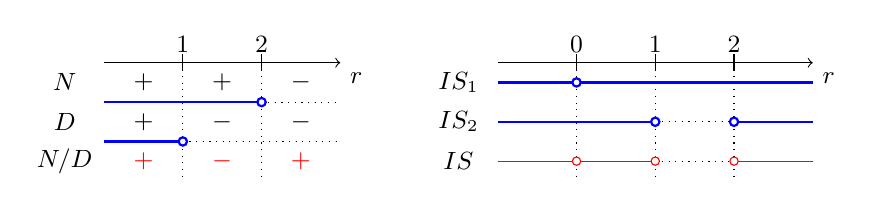
\begin{tikzpicture}[font=\small,x=10mm, y=10mm]

\draw[->] (0,0) -- (3,0) node [below right] () {$r$};
\draw[->] (5,0) -- (9,0) node [below right] () {$r$};

\foreach \x in {1,2,6,7,8}{
\draw(\x,3pt)--(\x,-3pt);
\begin{scope}[dotted]
\draw (\x,0) -- (\x,-1.5);
\draw (2,-.5) -- (3,-.5);
\draw (1,-1) -- (3,-1);
\draw (7,-.75) -- (8,-.75);
\draw (7,-1.25) -- (8,-1.25);
\end{scope}}

\node[above]  at (1,0) {$1$};
\node[above]  at (2,0) {$2$};
\node[above]  at (6,0) {$0$};
\node[above]  at (7,0) {$1$};
\node[above]  at (8,0) {$2$};

\begin{scope}[blue,thick]
\draw (0,-.5) -- (2,-.5);
\draw (1,-1) -- (0,-1);
\draw (5,-.25) -- (6,-.25);
\draw (5,-.25) -- (9,-.25);
\draw (5,-.75) -- (7,-.75);
\draw (8,-.75) -- (9,-.75);

\draw[fill=white] (2,-.5)circle (1.5pt);
\draw[fill=white] (1,-1)circle (1.5pt);
\draw[fill=white] (6,-.25)circle (1.5pt);
\draw[fill=white] (7,-.75)circle (1.5pt);
\draw[fill=white] (8,-.75)circle (1.5pt);
\end{scope}

\foreach \x in {4.5}{
\node  at (\x,-.25) {$IS_1$};
\node  at (\x,-.75) {$IS_2$};
\node  at (\x,-1.25) {$IS$};
}
\foreach \x in {-0.5}{
\node  at (\x,-.25) {$N$};
\node  at (\x,-.75) {$D$};
\node  at (\x,-1.25) {$N/D$};
}

\foreach \z in {.5,1.5}
\node  at (\z,-.25) {$+$};

\foreach \zi in {1.5,2.5}
\node  at (\zi,-.75) {$-$};

\node  at (2.5,-.25) {$-$};
\node  at (0.5,-.75) {$+$};

\begin{scope}[red]
\foreach \y in {-1.25}{
\foreach \ziv in {1.5}
	\node at (\ziv,\y) {$-$};
\foreach \zv in {.5,2.5}
\node at (\zv,\y) {$+$};
\draw (5,-1.25) -- (7,-1.25);
\draw (8,-1.25) -- (9,-1.25);
\draw[fill=white] (6,-1.25)circle (1.5pt);
\draw[fill=white] (7,-1.25)circle (1.5pt);
\draw[fill=white] (8,-1.25)circle (1.5pt);

}
\end{scope}
\end{tikzpicture}

\end{center}
ricaviamo $\IS_{2} = \{k \in \insR | k \ldots \ldots \ldots \vee k > \ldots \ldots \ldots \}$.
Dal grafico a destra inoltre otteniamo $\IS = \IS_{1} \cap \IS_{2} = \{ k \in \insR | k
\ldots \ldots \ldots \vee 0 < k < \ldots \ldots \vee k \ldots \ldots \ldots \}$.
\end{esercizio}

\begin{esercizio}
 \label{ese:3.92}
Assegnata l’equazione $(k + 1) x^{2} + (k + 3) x + k = 0$ stabilire per quale valore di $k$ una sua soluzione è $x =-1$. In tale caso determinare l’altra soluzione.

\emph{Traccia di svolgimento}:
Ricordiamo che un valore numerico è soluzione di un'equazione se sostituito all’incognita trasforma l’equazione in una uguaglianza vera.
Per questo motivo, sostituendo all’incognita il valore assegnato, il parametro $k$ dovrà verificare l’uguaglianza: $(k + 1) (- 1)^{2} + (k + 3) (- 1) + k = 0 \Rightarrow\ldots\ldots\ldots\ldots$
Sostituendo il valore di $k$ trovato, l’equazione diventa: $3 x^{2} + 5 x + 2 = 0$; l’altra soluzione può essere trovata o con la formula risolutiva, oppure
ricordando che $x_{1} + x_{2}=- \frac{b}{a}=- \frac{5}{3}$ da cui $x_{2}=\ldots\ldots$ o anche $x_{1} \cdot x_{2}=\frac{c}{a}=\frac{2}{3}$ da cui $x_{2}=\ldots\ldots$
\end{esercizio}

\begin{esercizio}
 \label{ese:3.93}
Giustificare la verità della seguente proposizione: “per qualunque valore assegnato al parametro $m$ l’equazione $(m-1) x^{2} + 2 m x + m + 1 = 0$
ha soluzioni reali distinte”.
Determinare inoltre $m$ affinché: a) $x_{1} + x_{2} = 1-\sqrt{3}$;\quad b) $ x_{1} \cdot x_{2} = \frac{12}{5}$;\quad c) $x_{1} + x_{2} = 1-x_{1} \cdot x_{2}$.
\end{esercizio}

\begin{esercizio}
 \label{ese:3.94}
Nell’equazione $7 x^{2} + (k-5) x-(k + 2) = 0$ determinare $k$ affinché le soluzioni siano reali; distingui i casi “reali coincidenti” e “reali distinte”.
Nel primo caso determina $x_{1} = x_{2} = \ldots \ldots$; nel secondo caso, determina $k$ affinché
\begin{enumeratea}
\item il prodotto delle soluzioni sia $- \frac{8}{3}$;
\item una soluzione sia nulla;
\item le soluzioni siano una il reciproco dell’altra, cioè: $x_{1} = \frac {1} {x_{2}}$;
\item la somma dei reciproci delle soluzioni sia $\frac{1} {2}$;
\item la somma delle soluzioni superi il loro prodotto di $2$.
\end{enumeratea}
\end{esercizio}

\begin{esercizio}
 \label{ese:3.95}
Verificare che nell’equazione $(2 m-3) x^{2}-(m + 2) x + 3 m-2 = 0$ si hanno due valori del parametro per cui le soluzioni sono reali coincidenti. Determina i due valori.
\end{esercizio}

\begin{esercizio}
 \label{ese:3.96}
Nell’equazione $x^{2}-2 (k + 2) x + (k^{2}-3 k + 2) = 0$ determinare $k$ affinché le soluzioni siano reali, con somma positiva e prodotto negativo.

\emph{Traccia di svolgimento}:
Il problema richiede tre condizioni alle quali deve soddisfare contemporaneamente il parametro, pertanto si formalizza con il sistema
$\left \{ \begin{array}{l} \Delta \geq 0 \\- \frac{b}{a} > 0\\
\frac{c}{a} < 0 \end{array}\right.$.
\end{esercizio}

\begin{esercizio}[\Ast]
 \label{ese:3.97}
Data l'equazione $x^{2}-2 x-k = 0$ determinare $k$ in modo che
\begin{enumeratea}
\item le soluzioni siano reali e distinte \quad $(\Delta>0)$;
\item la somma delle soluzioni sia $10 \quad (x_{1} + x_{2} = 10)$;
\item il prodotto delle soluzioni sia $10 \quad (x_{1} \cdot x_{2} = 10)$;
\item una soluzione sia uguale a $0$ \quad (sostituire $0$ alla $x$);
\item le radici siano opposte \quad $(x_{1} + x_{2} = 0)$;
\item le radici siano reciproche \quad $(x_{1} \cdot x_{2} = 1)$
\item le radici siano coincidenti \quad $(\Delta=0)$;
\item la somma dei quadrati delle radici sia $12 \quad \left(x_{1}^{2} + x_{2}^{2} = (x_{1} + x_{2})^{2}-2x_{1} x_{2} = 12\right)$;
\item la somma dei reciproci delle radici sia $-4 \quad \left(\frac{1}{x_{1}} + \frac{1}{x_{2}} = \frac{x_{1} +x_{2}}{x_{1} x_{2}} =-4 \right)$
\item la somma dei cubi delle radici sia $1$ \protect\\ $\left( x_{1}^{3} + x_{2}^{3} = (x_{1} + x_{2})^{3}-3x_{1}^{2} x_{2}-3x_{1} x_{2}^{2} = (x_{1} + x_{2})^{3}-3x_{1} x_{2} (x_{1} + x_{2}) = 1\right)$;
\item le radici siano entrambe negative $\left(\left\{\begin{array}{l} x_{1} \cdot x_{2} > 0 \\x_{1} + x_{2} < 0 \end{array}\right.\right)$.
\end{enumeratea}
\end{esercizio}

\begin{esercizio}[\Ast]
 \label{ese:3.98}
Data l'equazione $x^{2}-k x-1 = 0$ determinare $k$ in modo che
\begin{enumeratea}
\item le soluzioni siano coincidenti;
\item la somma delle radici sia $8$;
\item le radici siano opposte;
\item una radice sia $- \frac{1}{3}$;
\item il prodotto delle radici sia $-1$.
\end{enumeratea}
\end{esercizio}

\begin{esercizio}[\Ast]
 \label{ese:3.99}
Data l'equazione $x^{2} + (k + 1) x + k = 0$ determinate $k$ affinché l'equazione
\begin{enumeratea}
\item abbia una soluzione sia uguale a zero;
\item abbia soluzioni opposte;
\item non abbia soluzioni reali;
\item abbia le radici reciproche;
\item abbia le radici positive (regola di Cartesio).
\end{enumeratea}
\end{esercizio}

\begin{esercizio}[\Ast]
 \label{ese:3.100}
Data l'equazione $x^{2}-kx + 6 = 0$ determinate $k$ affinché
\begin{enumeratea}
\item abbia la somma delle radici uguale a $7$;
\item abbia le radici reali e opposte;
\item abbia la somma dei reciproci delle radici uguale a $-6$;
\item abbia una radice uguale a $- \frac{3}{2}$;
\end{enumeratea}
\end{esercizio}

\begin{esercizio}[\Ast]
 \label{ese:3.101}
Data l'equazione $x^{2} + (k + 1) x + k^{2} = 0$ determinare $k$ affinché
\begin{enumeratea}
\item abbia come soluzione $-1$;
\item abbia una soluzione doppia $(x_1 =x_2)$;
\item abbia le radici reciproche;
\item abbia una radice l'opposto della reciproca dell'altra $\left(x_1=-\frac{1}{x_2}\rightarrow x_1 \cdot x_2=-1\right)$;
\item abbia una radice nulla.
\end{enumeratea}
\end{esercizio}

\begin{esercizio}[\Ast]
 \label{ese:3.102}
Data l'equazione $kx^{2}-2kx + k-2 = 0$ determinare $k$ affinché
\begin{enumeratea}
\item abbia una radice nulla;
\item abbia la somma dei reciproci delle radici uguale a $1$;
\item abbia la somma dei quadrati delle radici uguale a $4$;
\item abbia la somma delle radici che superi di $5$ il loro prodotto.
\end{enumeratea}
\end{esercizio}

\begin{esercizio}[\Ast]
 \label{ese:3.103}
Data l'equazione $x (x-a) = \frac{a + x}{a + 2}$ determinate $a$ affinché
\begin{enumeratea}
\item una soluzione sia $1$;
\item l'equazione sia di primo grado;
\item una soluzione sia uguale al reciproco dell'altra;
\item la somma delle soluzioni sia il doppio del loro prodotto;
\item la somma dei quadrati delle soluzioni sia $0$;
\item la somma delle radici sia l'opposto del loro prodotto;
\item le soluzioni siano reali e distinte;
\item l'equazione sia spuria;
\item la somma dei cubi delle soluzioni sia nulla;
\item le soluzioni siano reali e discordi;
\item la somma dei reciproci dei cubi sia $1$.
\end{enumeratea}
\end{esercizio}

\begin{esercizio}[\Ast]
 \label{ese:3.104}
Data l'equazione $kx^{2}-(2k + 1) x + k-5 = 0$ determinare il valore di $k$ per il quale
\begin{enumeratea}
\item l'equazione ha soluzioni reali;
\item il prodotto delle radici sia $-2$;
\item la somma delle radici sia $1$;
\item una soluzione sia $-2$;
\item le soluzioni siano opposte;
\item la somma dei reciproci sia $3$;
\item le soluzioni siano reciproche;
\item una soluzione sia l'opposto del reciproco dell'altra;
\item la somma dei quadrati delle soluzioni sia $4$;
\item le radici siano concordi;
\item le radici siano entrambe negative;
\item la somma delle radici uguagli l'opposto del loro prodotto.
\end{enumeratea}
\end{esercizio}

\begin{esercizio}
 \label{ese:3.105}
 Per quale valore di $k \in \insR$ l'equazione $kx^{2}-x + k = 0$ non ammette soluzioni reali?
\[\boxA\; k \leq-\frac{1}{2} \vee k \geq + \frac{1}{2}\quad\boxB\; - \frac{1}{2} < k < \frac{1}{2}\quad\boxC\; k <-\frac{1}{2} \vee k > \frac{1}{2}\quad\boxD\; - \frac{1}{2} \leq k \leq \frac{1}{2}\]
\end{esercizio}

\begin{esercizio}
 \label{ese:3.106}
Per quale valore di $k \in \insR$ l'equazione $x^{2} + (k-2) x + 1 = 0$ ammette due soluzioni reali e distinte?
\[\boxA\quad k > 4\qquad\boxB\quad k = 0 \vee k = 4\qquad\boxC\quad 0 < k < 4\qquad\boxD\quad k < 0 \vee k > 4\]
\end{esercizio}

\begin{esercizio}
 \label{ese:3.107}
Per quale valore di $k$ l'equazione $(k-1) x^{2} + kx + (k + 1) = 0$ ha una soluzione nulla?
\[\boxA\quad k = 1\qquad\boxB\quad k = -1\qquad\boxC\quad k =0\qquad\boxD\quad \text{nesssun valore di }k\]
\end{esercizio}

\begin{esercizio}
 \label{ese:3.108}
Per quale valore di $k$ l'equazione $kx^{2} + \frac{1}{2} x + 1 = 0$ ha due soluzioni identiche?
\[\boxA\quad k = \frac{1}{4}\qquad\boxB\quad k = \frac{1}{16}\qquad\boxC\quad k = 2\qquad\boxD\quad \text{nesssun valore di }k\]
\end{esercizio}

\begin{esercizio}
 \label{ese:3.109}
Per quale valore di $k$ l'equazione $(k + 3) x^{2}-2x + k = 0$ ammette due soluzioni reciproche?
\[\boxA\quad k = 0\qquad\boxB\quad k = -3\qquad\boxC\quad \text{qualsiasi valore di }k\qquad\boxD\quad \text{nesssun valore di }k\]
\end{esercizio}

\begin{esercizio}
 \label{ese:3.110}
Per quale valore di $k$ l'equazione $(k + 1) x^{2}-kx-4 = 0$ ha una soluzione uguale a $2$?
\[\boxA\quad k = 4\qquad\boxB\quad k =-2\qquad\boxC\quad k = 0\qquad\boxD\quad k =-1\]
\end{esercizio}

\begin{esercizio}
 \label{ese:3.111}
Se l'equazione $(k + 1) x^{2}-kx-4 = 0$ ha una soluzione uguale a $2$ quanto vale l'altra soluzione?
\[\boxA\quad x = 0\qquad\boxB\quad x =-2\qquad\boxC\quad x = \frac{1}{2}\qquad\boxD\quad x = 2\]
\end{esercizio}

\begin{multicols}{2}
%===================================
\subsection*{3.9 - Problemi di secondo grado}

\begin{esercizio}[\Ast]
 \label{ese:3.112}
Il quadrato di un numero reale supera la metà del numero stesso di $ 5 $.
Determina i numeri reali che rendono vera la proposizione enunciata.
\end{esercizio}

\begin{esercizio}[\Ast]
 \label{ese:3.113}
Il prodotto della metà di un numero relativo con il suo successivo è $ 666 $.
Quali numeri verificano questa proprietà?
\end{esercizio}

\begin{esercizio}
 \label{ese:3.114}
Trova un numero positivo che addizionato al proprio quadrato dia come somma $ 156 $.
\end{esercizio}

\begin{esercizio}
 \label{ese:3.115}
Un numero addizionato al quadrato della sua metà, dà come risultato $ 120 $.
Trova il numero.
\end{esercizio}

\begin{esercizio}
 \label{ese:3.116}
Verifica che non esiste alcun numero reale tale che il quadrato del suo
doppio uguagli la differenza tra il triplo del suo quadrato e il quadrato
della somma del numero con $ 3 $.
\end{esercizio}

\begin{esercizio}[\Ast]
 \label{ese:3.117}
Due numeri naturali hanno rapporto $ 2/3 $ e somma dei loro quadrati $ 3757 $.
Individua i numeri che verificano questa proprietà.
\end{esercizio}

\begin{esercizio}[\Ast]
 \label{ese:3.118}
La somma dei quadrati di due numeri pari consecutivi è $ 580 $. Quali sono i
due numeri?
\end{esercizio}

\begin{esercizio}[\Ast]
 \label{ese:3.119}
Di due numeri naturali consecutivi si sa che la somma dei loro reciproci
è $ 9/20 $. Quali sono i due numeri?
\end{esercizio}

\begin{esercizio}[\Ast]
 \label{ese:3.120}
Di cinque numeri interi consecutivi si sa che la differenza tra il quadrato
della somma degli ultimi due numeri e la somma dei quadrati dei primi tre è
$ 702 $. Qual è il più piccolo di questi numeri?
\end{esercizio}

 \begin{esercizio}[\Ast]
 \label{ese:3.121}
La somma delle età di un padre con quella del figlio è $ 34 $. Sapendo che
l'età del padre aumentata di $ 8 $ anni dà il quadrato dell'età del figlio,
trovare le due età.
\end{esercizio}

\begin{esercizio}[\Ast]
 \label{ese:3.122}
Determina due numeri naturali sapendo che la somma tra il doppio del minore
ed il triplo del maggiore è $ 42 $ e che il rapporto tra la loro somma e il loro
prodotto è $ 5/12 $.
\end{esercizio}

\begin{esercizio}[\Ast]
 \label{ese:3.123}
Trova l'età di una persona sapendo che fra tre anni la sua età sarà
uguale al quadrato della quinta parte dell'età che aveva tre anni fa.
\end{esercizio}

\begin{esercizio}[\Ast]
 \label{ese:3.124}
Trova due numeri pari consecutivi tali che la somma del quadrato del minore
con il loro prodotto sia $ 544 $.
\end{esercizio}

\begin{esercizio}[\Ast]
 \label{ese:3.125}
Trova due numeri naturali sapendo che il minore supera di $ 2 $ la terza parte
del maggiore e che il quadrato del maggiore supera di $ 68 $ il quadrato del
doppio del minore.
\end{esercizio}

\begin{esercizio}[\Ast]
 \label{ese:3.126}
Da un segmento di $ 25\unit{cm} $ ne vogliamo ottenere due in modo che la somma dei
loro quadrati sia $ 337 $.
\end{esercizio}

\begin{esercizio}[\Ast]
 \label{ese:3.127}
In una frazione il numeratore e il denominatore hanno somma $ 14 $, mentre la
somma dei loro quadrati è $ 106 $. Qual è la frazione?
\end{esercizio}

\begin{esercizio}[\Ast]
 \label{ese:3.128}
Due navi partono contemporaneamente da uno stesso porto e arrivano alla
stessa destinazione dopo aver percorso sulla stessa rotta a velocità
costante $ 720\unit{miglia} $. Sapendo che una delle due navi viaggia con una velocità
di 1 nodo (1 miglio all'ora) superiore a quella dell'altra nave e che perciò
arriva 3 ore prima a destinazione, determina le velocità in nodi delle due
navi.
\end{esercizio}

\begin{esercizio}
 \label{ese:3.129}
Due navi che viaggiano su rotte perpendicolari a velocità costante si
incontrano in mare aperto. Sapendo che una delle navi viaggia a 15 nodi (1
nodo = 1 miglio all'ora), dopo quanto tempo le due navi si trovano alla
distanza di 40 miglia?
\end{esercizio}

\begin{esercizio}
 \label{ese:3.130}
Luca e Carlo bevono due aranciate in bottiglia. Nel tempo in cui Luca beve
11 sorsi, Carlo ne beve 8, ma due sorsi di Carlo equivalgono a tre di Luca.
Quando Carlo inizia a bere Luca ha già preso 4 sorsi. Dopo quanti sorsi di
Carlo le due bibite hanno lo stesso livello?
\end{esercizio}

\begin{esercizio}
 \label{ese:3.131}
Un maratoneta durante un allenamento fa due giri di un percorso di $ 22\unit{km} $
mantenendo in ciascun giro una velocità costante ma nel secondo giro la
velocità è inferiore di $ 0,5\unit{km/h} $ rispetto al primo giro. A quali velocità
ha corso se ha impiegato complessivamente 2 ore e un quarto?
\end{esercizio}

\begin{esercizio}[\Ast]
 \label{ese:3.132}
Un capitale di 12000 euro è depositato in banca a un certo tasso di interesse
annuale. Alla scadenza del primo anno gli interessi maturati vengono
ridepositati sullo stesso conto. Alla scadenza del secondo anno si ritira la
somma di 12854,70 euro. Qual è stato il tasso di interesse?
\end{esercizio}

\begin{esercizio}
 \label{ese:3.133}
In un rettangolo, se si aumenta di 2 metri la base e si riduce di un metro
l’altezza, la sua area aumenta di 4 metri quadrati. Se invece si riduce di
un metro la base e si aumenta di 2 metri l’altezza, l’area aumenta di 22
metri quadrati. Quali sono le dimensioni del rettangolo?
\end{esercizio}

\begin{esercizio}[\Ast]
 \label{ese:3.134}
Una ditta spende mensilmente 73500 in stipendi per i propri dipendenti.
Aumentando di 5 il numero dei dipendenti, ma riducendo l'orario di lavoro,
diminuisce a ciascuno lo stipendio di 200 e spende solamente 2500 in più per
gli stipendi. Quanti dipendenti aveva inizialmente la ditta e quanto
guadagnava ognuno di essi?
\end{esercizio}

\begin{esercizio}[\Ast]
 \label{ese:3.135}
Da un cartoncino rettangolare ($ ABCD $, come in figura) si vuole ritagliare un
quadrato ($ DEFG $) in modo che le due parti ottenute siano equivalenti.
Determinare la misura del lato del quadrato sapendo che
$\overline {EC} = 6\unit{cm} $ e $\overline {AG} = 4\unit{cm}$.
\begin{center}
 % (c) 2013 Claudio Carboncini - claudio.carboncini@gmail.com
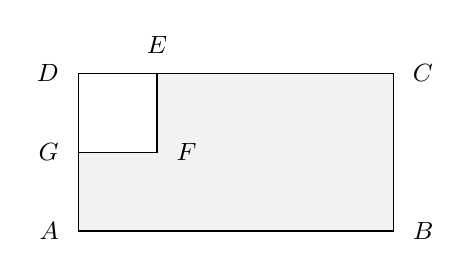
\begin{tikzpicture}[x=10mm,y=10mm,font=\small]

  \fill[fill=gray!10] (1,1) rectangle (5,3);
  \fill[fill=white] (1,3) rectangle (2,2);
  \draw (1,1) rectangle (5,3);
  \draw (1,3) rectangle (2,2);
  \node [label={[name=label node]left:$A$}] at (1,1) {};
  \node [label={[name=label node]left:$D$}] at (1,3) {};
  \node [label={[name=label node]right:$C$}] at (5,3) {};
  \node [label={[name=label node]right:$B$}] at (5,1) {};
  \node [label={[name=label node]left:$G$}] at (1,2) {};
  \node [label={[name=label node]right:$F$}] at (2,2) {};
  \node [label={[name=label node]above:$E$}] at (2,3) {};

%  \foreach \x in {1,5}
%    \foreach \y in {1,3}
%      \filldraw[fill=black, draw=black]  (\x,\y) circle (1pt);
%      \filldraw[fill=black, draw=black]  (1,2) circle (1pt);
%      \filldraw[fill=black, draw=black]  (2,3) circle (1pt);

\end{tikzpicture}

\end{center}
\end{esercizio}

\begin{esercizio}[\Ast]
 \label{ese:3.136}
Un terreno a forma rettangolare di $6016\unit{m^2}$ viene recintato con un muro lungo
$350\unit{m}$. Quali sono le dimensioni del rettangolo?
\end{esercizio}

\begin{esercizio}[\Ast]
 \label{ese:3.137}
Determinare sul segmento $ AB $ di misura $ 5\unit{m} $ un punto $ P $ tale che il rettangolo
delle due parti sia equivalente al quadrato di lato $ 2\unit{m} $. Rappresenta con un
disegno le soluzioni.
\end{esercizio}

\begin{esercizio}[\Ast]
 \label{ese:3.138}
Calcolare perimetro e area del triangolo $ ABC $ isoscele sulla base $ AB $ sapendo
che la differenza tra la base e l’altezza ad essa relativa è $ 0,5\unit{m} $ e tale
è anche la differenza tra il lato $ CB $ e la base stessa.
\end{esercizio}

\begin{esercizio}[\Ast]
 \label{ese:3.139}
La superficie del rettangolo $ ABCD $ supera di $ 119\unit{m^2} $ la superficie del quadrato
costruito sul lato minore $ AD $. Determinare il perimetro e la misura della
diagonale sapendo che i $ 7/10 $ del lato maggiore AB sono uguali ai $ 12/5 $ del
lato minore.
\end{esercizio}

\begin{esercizio}[\Ast]
 \label{ese:3.140}
Nel trapezio rettangolo $ ABCD $, il rapporto tra la base maggiore $ AB $ e la base
minore $ CD $ è $ 8/5 $, il lato obliquo forma con $ AB $ un angolo di $ 45\grado $. Determinare
il perimetro sapendo che l’area è $312\unit{m^2}$.
\end{esercizio}

\begin{esercizio}[\Ast]
 \label{ese:3.141}
Determina il perimetro di un rombo che ha l'area di $24\unit{m^2}$ e il rapporto tra
le diagonali $ 4/3 $.
\end{esercizio}

\begin{esercizio}[\Ast]
 \label{ese:3.142}
Un rettangolo $ ABCD $ ha il perimetro di $ 48\unit{cm} $ e l'area di $ 128\unit{cm^2} $. A una certa
distanza $x$ dal vertice $ A $ sui due lati $ AD $ e $ AB $ si prendono rispettivamente i
punti $ P $ e $ Q $. Alla stessa distanza $ x $ dal vertice $ C $ sui lati $ CB $ e $ CD $ si
prendono rispettivamente i punti $ R $ e $ S $. Sapendo che il rapporto tra l'area
del rettangolo $ ABCD $ e l'area del quadrilatero $ PQRS $ è $ 32/23 $ calcola la
distanza $x$.
\end{esercizio}

\begin{esercizio}
 \label{ese:3.143}
Un trapezio rettangolo ha la base minore di $ 9|unit{cm} $, l'altezza i $ 2/9 $ della base
maggiore e l'area di $20 + 9 \sqrt{2}\unit{cm^{2}}$. Determina la misura della base maggiore.
\end{esercizio}

\begin{esercizio}[\Ast]
 \label{ese:3.144}
Da un quadrato di $ 32\unit{cm} $ di lato vengono ritagliati due triangoli rettangoli
come descritti in figura. Calcola la misura di $ x $,
inferiore alla metà del lato del quadrato, in modo che l’area totale dei
due triangoli evidenziati sia pari a $ 344\unit{cm^2} $.
\begin{center}
 % (c) 2013 Claudio Carboncini - claudio.carboncini@gmail.com
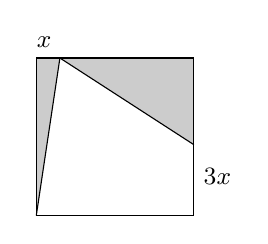
\begin{tikzpicture}[x=10mm,y=10mm,font=\small]

  \fill[fill=gray!40] (1,1) -- (1,3) -- (1.3,3);
  \fill[fill=gray!40] (1.3,3) -- (3,3) -- (3,1.9);
  \draw (1,1) rectangle (3,3);
  \draw (1.3,3)--(1,1);
  \draw (3,1.9)--(1.3,3);
  \node (x) at (1.1,3.2) {$x$};
  \node (h) at (3.3,1.5) {$3x$};

\end{tikzpicture}

\end{center}
\end{esercizio}

\begin{esercizio}[\Ast]
 \label{ese:3.145}
Il rettangolo $ ABCD $ ha l’area di $ 558\unit{cm^2} $ e il lato $ DC $ di $ 18\unit{cm} $. Lo si
vuole trasformare in un nuovo rettangolo $ AEFG $ accorciando l’altezza di una quantità $ 5x $ e allungando la base di
una quantità $ 4x $ in modo che il nuovo rettangolo $ AEFG $ che abbia l’area di
$ 228\unit{cm^2} $. Determina la quantità $ x $ necessaria a compiere la trasformazione
richiesta.
\end{esercizio}

\begin{esercizio}[\Ast]
 \label{ese:3.146}
Il rettangolo $ AEFG $ ha l’area di $ 768\{cm^2\} $ e l’altezza $ AG $ di $ 24\unit{cm} $. Si
vuole allungare l’altezza di una quantità
$ x $ e accorciare la base di una quantità doppia $ 2x $ in modo da ottenere un
secondo rettangolo $ ABCD $ che abbia l’area di $ 702\unit{cm^2} $. Determina $ x $.
\end{esercizio}

\begin{esercizio}
 \label{ese:3.147}
Un trapezio isoscele di area $ 144\unit{cm^2} $ ha la base maggiore che supera di $ 10\unit{cm} $
la base minore che a sua volta supera di $ 10\unit{cm} $ l'altezza. Determina il perimetro del trapezio.
\end{esercizio}

\begin{esercizio}[\Ast]
 \label{ese:3.148}
Il rettangolo $ ABCD $ ha l’area di $ 240\unit{cm^2} $ e l’altezza $ AD $ di $ 12\unit{cm} $. Si
vuole trasformare il rettangolo in un triangolo $ AEF $ allungando l’altezza di una quantità $ 3x $ e accorciando la
base di una quantità $ x $ (vedi figura) in modo che il nuovo triangolo $ AEF $ abbia l’area di $ 162\unit{cm^2} $.
\begin{center}
 % (c) 2013 Claudio Carboncini - claudio.carboncini@gmail.com
\begin{tikzpicture}[x=10mm,y=10mm,font=\small]
  \draw (1,1) rectangle (5,2); %ABCD
  \draw (1,1)--(2.6,4.4); %AF
  \draw (4.2,1)--(2.6,4.4); %EF
  \draw [dashed] (2.6,4.4) -- (2.6,2);
  \draw [dotted] (2.6,2) -- (2.6,1);
  \node (x) at (4.6,.7) {$x$};
  \node (h) at (2.3,3) {$3x$};
  \node [label={[name=label node]below left:$A$}] at (1,1) {};
  \node [label={[name=label node]above left:$D$}] at (1,2) {};
  \node [label={[name=label node]above right:$C$}] at (5,2) {};
  \node [label={[name=label node]below right:$B$}] at (5,1) {};
  \node [label={[name=label node]below:$E$}] at (4.2,1) {};
  \node [label={[name=label node]above:$F$}] at (2.6,4.4) {};

%  \foreach \x in {1,5}
%    \foreach \y in {1,2}
%      \filldraw[fill=black, draw=black]  (\x,\y) circle (1pt);
%      \filldraw[fill=black, draw=black]  (2.6,4.4) circle (1pt);
%      \filldraw[fill=black, draw=black]  (4.2,1) circle (1pt);

\end{tikzpicture}

\end{center}
\end{esercizio}

\begin{esercizio}[\Ast]
 \label{ese:3.149}
La piramide di Cheope è a base quadrata ed ha una superficie totale pari a
$ 135700\unit{m^2} $. Sapendo che l’apotema della piramide misura $ 180 $ metri, si
calcoli la lunghezza del lato di base.
\end{esercizio}

\begin{esercizio}[\Ast]
 \label{ese:3.150}
Un container a forma di parallelepipedo a base quadrata ha una superficie
totale pari a $ 210\unit{m^2} $. L’altezza è il doppio del lato di base diminuito di
$ 2 $ metri. Trovare la lunghezza del lato di base.
\end{esercizio}

\subsection*{3.10 - Problemi con un parametro}

\begin{esercizio}
 \label{ese:3.151}
Sul prolungamento dei lati $ AB $, $ BC $, $ CD $, $ DA $ del quadrato $ ABCD $ prendi rispettivamente i punti $ Q $, $ R $, $ S $, $ P $ in modo che $ QB=RC=SD=PA $. Dimostra che $ PQRS $ è un quadrato; nell’ipotesi che sia $AB = 3\unit{m}$ determina $\overline {AP}$ in modo che l’area di $ PQRS $ sia $ k $, con $ k $ reale positivo.
\begin{center}
 % (c) 2013 Claudio Carboncini - claudio.carboncini@gmail.com
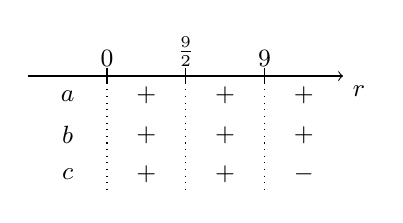
\begin{tikzpicture}[font=\small,x=10mm, y=10mm]

\draw[->] (0,0) -- (4,0) node [below right] () {$r$};

\foreach \x in {1,2,3}{
\draw(\x,3pt)--(\x,-3pt);
\begin{scope}[dotted]
\draw (\x,0) -- (\x,-1.5);
\end{scope}}

\node[above]  at (1,0) {$0$};
\node[above]  at (2,0) {$\frac 9 2$};
\node[above]  at (3,0) {$9$};

\foreach \x in {0.5}{
\node  at (\x,-.25) {$a$};
\node  at (\x,-.75) {$b$};
\node  at (\x,-1.25) {$c$};
}

\foreach \z in {1.5,2.5,3.5}
\node  at (\z,-.25) {$+$};

\foreach \zi in {1.5,2.5,3.5}
\node  at (\zi,-.75) {$+$};

\node  at (1.5,-1.25) {$+$};
\node  at (2.5,-1.25) {$+$};
\node  at (3.5,-1.25) {$-$};
\end{tikzpicture}

\end{center}
\emph{Svolgimento}:
per dimostrare che $ PQRS $ è un quadrato dobbiamo dimostrare che i lati sono
congruenti e che gli angoli sono retti. Se si pone $\overline{AP} = x$ con $x > 0$.
$\Area(PQRS)= \overline {PQ}^{2} = \overline {PA}^{2} + \overline{AQ}^{2}$per il teorema di Pitagora.
Verifica che si ottiene l’equazione risolvente $2 x^{2} + 6 x + (9-k) = 0$. Poiché vogliamo soluzioni reali positive, discuti l’equazione con il metodo di Cartesio. Il discriminante è $\Delta = 36-8 (9-k)$ pertanto l'equazione ammette soluzioni reali per $k \geq \frac{9}{2}$. Dal segno dei coefficienti, essendo i primi due coefficienti positivi si ha una permanenza e quindi una radice negativa che non è accettabile. Per ottenere una soluzione positiva ci deve essere una variazione di segno negli ultimi due coefficienti, in altre parole $9-k$ deve essere negativo cioè $9-k < 0 \rightarrow k > 9$. Pertanto il problema ha soluzioni per $k > 9$.
\end{esercizio}

\begin{esercizio}
 \label{ese:3.152}
Nel trapezio rettangolo $ ABCD $ di base maggiore $ BC $, la diagonale $ AC $ è bisettrice dell’angolo $B \widehat {C} D$. Posto $\overline {AB} = 1\unit{m}$, determina la base maggiore in modo che sia $ 2k $ il perimetro del trapezio. Imposta dati e obiettivo del problema.
\begin{center}
 % (c) 2013 Claudio Carboncini - claudio.carboncini@gmail.com
\begin{tikzpicture}[x=10mm,y=10mm,font=\small]

  \coordinate(a) at (0,2.598);%il punto A
  \coordinate(b) at (0,0);%il punto B
  \coordinate(c) at (4.5,0);%il punto C
  \coordinate(d) at (3,2.598);%il punto D
  \coordinate (h) at ($(a)!(d)!(c)$);%trova le coordinate della proiezione di D su a--c
  \coordinate (h1) at ($(a)!{1/2}!(h)$);
  \coordinate (h2) at ($(h)!{1/2}!(c)$);
  \coordinate (a1) at ($(a)!{1/2}!(d)$);
  \coordinate (d1) at ($(d)!{1/2}!(c)$);
  \draw (a) -- (b)  -- (c) -- (d) -- cycle;%disegna il trapezio
  \draw [] (d) -- (h);%perpendicolare da D a a--c
  \draw [] (a) -- (c);%la diagonale del trapezio
  \draw (h1) node {$//$} ;
  \draw (h2) node {$//$} ;
  \draw (a1) node {$\times$} ;
  \draw (d1) node {$\times$} ;
  \draw (4.1,0.4) node {$\bullet$} ;
  \draw (3.95,0.12) node {$\bullet$} ;
  \node [label={[name=label node]above:$A$}] at (a) {};
  \node [label={[name=label node]below:$B$}] at (b) {};
  \node [label={[name=label node]below:$C$}] at (c) {};
  \node [label={[name=label node]above:$D$}] at (d) {};
  \node [label={[name=label node]below:$H$}] at (h) {};

\end{tikzpicture}

\end{center}
\emph{Svolgimento}: poniamo $\overline {BC} = x$. Dall’informazione che la diagonale $ AC $ è bisettrice dell’angolo $B \widehat {C} D$, possiamo dimostrare che $ ADC $ è un triangolo isoscele sulla base $ AC $. L’equazione risolvente sarà determinata dalla relazione tra i lati che esprime il perimetro del trapezio. Dobbiamo quindi esprimere $\overline {DC}$ in funzione di $ x $. Traccia l’altezza $ DH $ del triangolo isoscele $ ADC $ e dopo aver dimostrato la similitudine di $ ABC $ con $ DHC $, osserva che si ha $DC : AC = HC : BC$ poiché $HC = \frac{1}{2} AC$ si ha $\frac{1}{2} \overline {AC}^{2} = \overline {DC} \cdot \overline {BC}$ da cui si può ricavare la misura di $ DC = \frac{1}{2} \frac{AC^{2}}{BC}$. Dato che $\overline {AC}^{2}=1+x^2$, per il teorema di Pitagora applicato al triangolo $ ABC $, quindi $ DC = \frac{1 + x^2} {2 x} $ L’equazione parametrica risolvente è $2 x^{2} + x \cdot (1-2 k) + 1 = 0$ con $x > 0$ che può essere discussa con il metodo di Cartesio.
\end{esercizio}

\begin{esercizio}
 \label{ese:3.153}
Il quadrilatero $ ABCD $ ha le diagonali perpendicolari ed è inscritto in una circonferenza; sapendo che $\overline{AB} = 5a$; $\overline {AE} = 3 a$; $2 p_{BCA} = \frac{5}{2} \cdot \overline {BD}$, essendo $ E $ punto d’incontro delle diagonali, determinate la misura delle diagonali. Poni $\overline {CE} = x$.
\end{esercizio}

\begin{esercizio}
 \label{ese:3.154}
Il rettangolo $ ABCD $ ha i lati $ AB $ e $ BC $ che misurano rispettivamente $ a $ e $ 3a $ (con $ a\geq 0 $). Prolunga il lato $ AB $ di due segmenti congruenti $ BN $ e $ AM $ e sia $ V $ il punto di intersezione delle retta $ MD $ e $ CN $. Posto $\overline {BN} = x$, determina la misura della base $ MN $ del triangolo $ MVN $ in modo che la sua area sia $ k $ volte l’area del rettangolo assegnato.
\end{esercizio}

\begin{esercizio}
 \label{ese:3.155}
Due numeri reali hanno come somma $ a $ con $(a \in \insR_{0})$; determinare i due numeri in modo che il loro prodotto sia $ k $ con $(k \in \insR_{0})$. Quale condizione si deve porre sull’incognita? Per quale valore del parametro i due numeri soluzione sono uguali?
\end{esercizio}

\begin{esercizio}
 \label{ese:3.156}
In un triangolo rettangolo l’altezza $ AH $ relativa all’ipotenusa $ BC $ misura $ 1\unit{m} $ e $A \widehat {B} C = 60\grado$. Determinare sulla semiretta $ AH $, esternamente al triangolo, un punto $ P $ in modo che sia $ k $ la somma dei quadrati delle distanze di $ P $ dai vertici del triangolo. Quale condizione va imposta al parametro $ k $ perché il problema abbia significato?
\end{esercizio}

\begin{esercizio}
 \label{ese:3.157}
$\overline {AB} = 16 a$; $\overline {BC} = 2 a \sqrt{14}$ rappresentano le misure dei lati del rettangolo $ ABCD $; determinare un punto $ P $ del segmento $ AB $ tale che la somma dei quadrati delle sue distanze dai vertici $ C $ e $ D $ sia uguale al quadrato della diagonale $ DB $. Posto $\overline {AP} = x$ quale delle seguenti condizioni deve rispettare la soluzione? Dopo aver risolto il problema spiegare il significato delle soluzioni ottenute.
\end{esercizio}

\begin{esercizio}
 \label{ese:3.158}
Ad una sfera di raggio $ 1\unit{m} $ è circoscritto un cono il cui volume è $ k $ volte il volume della sfera. Determina l’altezza del cono.
\begin{center}
 % (c) 2013 Claudio Carboncini - claudio.carboncini@gmail.com
\begin{tikzpicture}[x=10mm,y=10mm,font=\small,scale=1.3]

  \coordinate(a) at (0,0);%il punto A
  \coordinate(v1) at (70:5);%il punto V1
  \coordinate(o) at (35:1.5);%il centro del cerchio O
  \coordinate(h) at (1.23,0);%il punto H
  \coordinate (b) at (2.46,0);%il punto B
  \coordinate(v2) at (1.23,6);%il punto v2
  \coordinate (v) at (intersection of a--v1 and h--v2);
  \coordinate (c) at ($(v)!(o)!(b)$);%trova le coordinate della proiezione di o su v--b
  \draw[] (o) circle (0.86);%disegna il cerchio di centro
  \draw[] (v) -- (a) -- (b) -- cycle;%disegna v2--h--a
  \draw[dashed] (v) -- (h);%disegna v--h
  \draw[dashed] (o) -- (c);%disegna o--c
  \draw (h) ellipse (1.23cm and 0.4cm);
  \node [label={[name=label node]above:$V$}] at (v) {};
  \node [label={[name=label node]left:$A$}] at (a) {};
  \node [label={[name=label node]below:$H$}] at (h) {};
  \node [label={[name=label node]right:$B$}] at (b) {};
  \node [label={[name=label node]left:$O$}] at (o) {};
  \node [label={[name=label node]right:$C$}] at (c) {};
\begin{comment}
  \coordinate (h2) at ($(h)!{1/2}!(c)$);
  \coordinate (a1) at ($(a)!{1/2}!(d)$);
  \coordinate (d1) at ($(d)!{1/2}!(c)$);
  \draw (a) -- (b)  -- (c) -- (d) -- cycle;%disegna il trapezio
  \draw [] (d) -- (h);%perpendicolare da D a a--c
  \draw [] (a) -- (c);%la diagonale del trapezio
  \draw (h1) node {$//$} ;
  \draw (h2) node {$//$} ;
  \draw (a1) node {$\times$} ;
  \draw (d1) node {$\times$} ;
  \draw (4.1,0.4) node {$\bullet$} ;
  \draw (3.95,0.12) node {$\bullet$} ;
\end{comment}
\end{tikzpicture}

\end{center}

\emph{Dati}: $ \overline {OC} = 1 $, $ \overline {OC} = \overline {OH} $, $ OC \perp VB $,\protect\\ $ \overline {BC} = \overline {BH} $, $ \overline {AH} = \overline {HB} $, $ VH \perp AB $,\protect\\ $ \text{Volume(cono)} = k \cdot \text{Volume(sfera)} $.

\emph{Obiettivo}: $\overline {VH}$

\emph{Svolgimento}: Poniamo $\overline {VO} = x$ con $x > 0$ da cui $\overline {VH}= \overline {VO} + \overline {OH} = x + 1$.

Ricordiamo che $V\text{(cono)} = \frac{1}{3} \pi \overline {HB}^{2} \cdot \overline {VH}$ e $V\text{(sfera)} = \frac{4}{3} \pi \overline {CO}^{3}$. Per impostare l’equazione risolvente dobbiamo cercare di esprimere $\overline {HB}^{2}$ in funzione di $ x $. Verifica che dalla similitudine di $ VOC $ con $ VHB $ si deduce: $\overline {HB} : \overline {OC} = \overline {VH} : \overline{VC}$ quindi $\overline {HB} = \frac{\overline {OC} \cdot \overline
{VH}}{\overline {VC}}$; dobbiamo ancora ricavare $\overline {VC}$ che per il teorema di Pitagora su $ VCO $ è \ldots Sostituendo tutti gli elementi trovati nella relazione che lega il volume del cono con il volume della sfera, verifica che si ottiene $x^{2} + 2 x (1-2 k) + 4 k = 0$ con $x > 0$, da discutere con il metodo di Cartesio.
\end{esercizio}

\end{multicols}
\begin{esercizio}[\Ast]
 \label{ese:3.159}
 Scheda di ripasso sulle equazioni
\begin{enumerate}
	\item L'equazione $25x^{2} + 1 = 0$ ha per soluzioni:

\boxA\quad $ x = \pm 5 $\qquad \boxB\quad $x = \pm \frac{1}{5}$\qquad\boxC\quad $x = 4 \vee x = 1$\qquad\boxD\quad non ha soluzioni reali

	\item L'equazione $16x^{2} + x = 0$ ha per soluzioni:

\boxA\quad $ x = 4 \vee x = 1 $\quad \boxB\quad $x = \pm \frac{1}{4}$\quad\boxC\quad $x =-\frac{1}{16} \vee x = 0$\quad\boxD\quad non ha soluzioni reali

	\item L'equazione $4x^{2}-9x = 0$ ha per soluzioni:

\boxA\quad $ x = \pm \frac{3}{2} $\qquad \boxB\quad $x = \pm \frac{9}{4}$\qquad\boxC\quad $x = \frac{3}{2} \vee x = 0$\qquad\boxD\quad $x = \frac{9}{4} \vee x = 0$

	\item L'equazione $9x^{2} + 6x + 1 = 0$ ha per soluzioni:

\boxA\quad $x = \pm 3$\qquad\boxB\quad $x = \pm \frac{1}{3}$\qquad\boxC\quad $x =-\frac{1}{3}$ doppia\qquad\boxD\quad non ha soluzioni reali

	\item L'equazione $x^{2}-6x + 36 = 0$ ha per soluzioni:

\boxA\quad $x = \pm 6$\qquad\boxB\quad $x = \pm \sqrt{6}$\qquad\boxC\quad $x =6$ doppia\qquad\boxD\quad non ha soluzioni reali

	\item Quale di queste equazioni ammette una soluzione doppia $ x=3 $?

\boxA\quad $2x^{2}-12x + 18 = 0$\quad\boxB\quad $9-x^{2} = 0$\quad\boxC\quad $x^{2} + 6x + 9 = 0$\quad\boxD\quad $ 3x^{2} + 9x = 0 $

	\item Quale equazione di secondo grado si ottiene con soluzioni $ x_1=1 $ e $ x_2=3 $?

\boxA\quad $x^{2} + x-1 = 0$\quad\boxB\quad $x^{2}-4x + 3 = 0$\quad\boxC\quad $x^{2}-4x-3 = 0$\quad\boxD\quad $ x^{2} + 4x-3 = 0 $

	\item Il polinomio$x^{2} + 5x + 6$ può essere scomposto in:

\boxA\; $(x + 2) (x-3)$\quad\boxB\; $(x + 5) (x + 1)$\quad\boxC\; $(x-2) (x-3)$\quad\boxD\; nessuna delle risposte precedenti

	\item Una delle soluzioni dell'equazione $x^{2}-(\sqrt{2} + 1) x + \sqrt{2} = 0$ è $\sqrt{2}$, quanto vale l'altra?

\boxA\quad $ - \sqrt{2} $\qquad \boxB\quad $\frac{1}{\sqrt{2}}$\qquad\boxC\quad $\sqrt{2} + 1$\qquad\boxD\quad $1$

	\item Per quale valore di $ k $ l'equazione $(2k-1) x^{2} + (2k + 1) x + k-2 = 0$ diventa di I° grado?

\boxA\quad $k = \frac{1}{2}$\qquad \boxB\quad $k =-\frac{1}{2}$\qquad\boxC\quad $k = 2$\qquad\boxD\quad $k = 0$

	\item L'equazione $4m^{2} x^{2}-5mx + 1 = 0$ con parametro $ m $ ha per soluzioni:

\boxA\; $x = m \vee x = 4m$\quad \boxB\; $x = \frac{1}{m} \vee x = \frac{1}{4m}$\quad\boxC\; $x = 64m \vee x = 1$\quad\boxD\; $x = m \vee x = \frac{1}{4}$

	\item L’equazione di secondo grado $x^{2} + (a + 1) x + a = 0$ con $ a $ parametro reale ha come soluzioni:

\boxA\; $x = 1 \vee x = a$\quad \boxB\; $x = a-1 \vee x = 1$\quad\boxC\; $x =-a \vee x =-1$\quad\boxD\; $x = a + 1 \vee x = a$

	\item L’equazione $x^{2} + (t-2) = 0$ con $ t $ parametro reale ammette soluzioni reali per:

\boxA\quad $t \leq 2$\qquad \boxB\quad $t \geq 2$\qquad\boxC\quad $t < 2$\qquad\boxD\quad nessuna delle risposte precedenti

	\item Quanto vale il prodotto delle soluzioni dell'equazione $x^{2}-6a^{2} x + 8a^{4} = 0$?

\boxA\quad $8a^{4}$\qquad \boxB\quad $8a^{2}$\qquad\boxC\quad $6a^{2}$\qquad\boxD\quad non esiste

	\item Il polinomio $x^{2} + (m-2) x-2m$ con $ m $ parametro reale può essere scomposto in:

\boxA\; $(x + m) (x + 1)$\quad\boxB\; $(x + m) (x-2)$\quad\boxC\; $(x + m) (x + 2)$\quad\boxD\; $(x-m) (x-2)$

	\item L’equazione $x^{2} + (k-1) x = 0$ con $ k $ parametro reale:

\boxA\; non ha soluzioni reali\quad\boxB\; ha una soluzione uguale a zero

\boxC\; due soluzioni reali coincidenti per $ k=0 $\quad\boxD\;soluzioni reali e distinte per $ k=1 $

	\item L’equazione $x^{2} + 2x + k-2 = 0$ con $ k $ parametro reale:

\boxA\quad ha due soluzioni reali coincidenti per $ k=3 $

\boxB\quad ha due soluzioni reali coincidenti per $ k=1 $

\boxC\quad ha una soluzione nulla per $k =-2$

\boxD\quad ha soluzioni reali e distinte per $k \neq 3$

	\item L’equazione $x^{2} + m^{2} + 1 = 0$ con $m$ parametro reale:

\boxA\; ammette due soluzioni reali e opposte\quad\boxB\; ammette due soluzioni coincidenti

\boxC\; non ammette soluzioni reali\quad\boxD\; ammette due soluzioni negative

	\item L’equazione $2x^{2} + k^{2} = 0$ con $k$ parametro reale ammette:

\boxA\; due soluzioni reali e distinte\quad\boxB\; due soluzioni reali solo se $k>0$

\boxC\; soluzioni coincidenti per $k = 0$\quad\boxD\; nessuna delle risposte precedenti è corretta

	\item L’equazione $tx^{2}-1 = 0$

\boxA\; ha come soluzioni $x_{1} = 0 \vee x_{2} = 1-t$\quad\boxB\; ammette sempre soluzioni reali

\boxC\; ammette soluzioni reali per $t > 0$\quad\boxD\; ha come soluzioni $x = \pm t$

\end{enumerate}
\end{esercizio}

\subsection{Risposte}
%\begin{multicols}{2}
\paragraph{3.1.} c)~$x_{1}=+4 \vee x_{2}=-4$,\quad f)$\emptyset$,\quad i)~$x_{1} = \sqrt{3} \vee x _{2} = - \sqrt{3}$,\quad l)~$\emptyset$.

\paragraph{3.2.} c)~$x_{1,2} = \frac{\pm \sqrt{15}}{5}$,\quad f)~$x_{1,2} = 0$,\quad i)~$x_{1,2} = \pm 7$,\quad l)~$x_{1,2} = \pm 2$.

\paragraph{3.3.} c)~$x_{1,2} = \pm 5$,\quad f)~$x_{1,2} = \pm \frac{1}{3}$,\quad i)~$x_{1,2} = \pm \frac{\sqrt{6}}{6}$,\quad l)~$x_{1,2} = \pm 2$.

\paragraph{3.4.} c)~$\emptyset$,\quad f)~$x_{1,2} = \pm 3 \sqrt{2}$,\quad i)~$x_{1,2} = \pm \sqrt{10}$,\quad l)~$x_{1,2} = \pm \frac{\sqrt{6}}{2}$.

\paragraph{3.5.} b)~$x_{1} = 0 \vee x_{2} = \frac{2}{3}$,\quad c)~$x_{1} = 0 \vee x_{2} = - \frac{2}{7}$,\quad e)~$x_{1} = 0 \vee x_{2} = - 5$.

\paragraph{3.6.} a)~$x_{1} = 0 \vee x_{2} = 2$,\quad c)~$x_{1} = 0 \vee x_{2} = \frac{1}{2}$,\quad e)~$x_{1} = 0 \vee x_{2} = \frac{5}{6}$.

\paragraph{3.7.} a)~$x_{1} = 0 \vee x_{2} = 2$,\quad c)~$x_{1} = 0 \vee x_{2} = 5$,\quad e)~$x_{1} = 0 \vee x_{2} = - 0,2$.

\paragraph{3.8.} a)~$x_{1} = 0 \vee x_{2} = 2$,\quad c)~$x_{1} = 0 \vee x_{2} = - \sqrt{2}$,\quad e)~$x_{1} = 0 \vee x_{2} = \frac{2}{5}$.

\paragraph{3.9.} a)~$x_{1} = 0 \vee x_{2} = \frac{4}{9}$,\quad c)~$x_{1} = 0 \vee x_{2} = - 2$,\quad e)~$x_{1} = 0 \vee x_{2} = 7$.

\paragraph{3.10.} a)~$x_{1} = 0 \vee x_{2} = - \frac{6}{11}$,\quad b)~$x_{1} = 0 \vee x_{2} = 6$,\quad c)~$x_{1} = 0 \vee x_{2} = 1$,\quad d)~$x_{1} = 0 \vee x_{2} = 4$.

\paragraph{3.11.} c)~$x_{1} = 0 \vee x_{2} = - (\sqrt{2} + \sqrt{5})$.

\paragraph{3.12.} a)~$x_{1} = 2 \vee x_{2} = 3$,\quad b)~.$x_{1} =-5 \vee x_{2} = 4$,\quad c)~$x_{1,2} = \frac{3 \pm \sqrt{21}}{7}$,\quad d)~$\emptyset$.

\paragraph{3.13.} a)~$x_{1} =-6 \vee x_{2} = 7$,\quad b)~$x_{1} = x_{2} = 5$,\quad c)~$x_{1} = 1 \vee x_{2} = \frac{5}{2}$,\quad d)~$x_{1} =-1 \vee x_{2} = \frac{1}{3}$.

\paragraph{3.14.} a)~$x_{1,2} = \frac{\sqrt{5} \pm \sqrt{13}}{4}$,\quad b)~$x_{1,2} = \sqrt{3} \pm \sqrt{7}$,\quad c)~$x_{1,2} = \frac{3 \pm \sqrt{17}}{2}$,\quad d)~$x_{1} =-\sqrt{2} \vee x_{2} = \frac{3 \sqrt{2}}{2}$.

\paragraph{3.15.} a)~$x_{1} =-\frac{3}{2} \vee x_{2} = \frac{3}{4}$,\quad b)~$x_{1} = \frac{1}{8} \vee x_{2} = \frac{1}{2}$,\quad c)~$\emptyset$,\quad d)~$x_{1,2} = \frac{\sqrt{5} \pm \sqrt{5 + 4 \sqrt{5}}}{2}$.

\paragraph{3.16.} a)~$x_{1,2} = \frac{5 \pm \sqrt{13}}{2}$,\quad b)~$\emptyset$,\quad c)~$x_{1,2} = 2 \pm \sqrt{13}$,\quad d)~$x_{1,2} =-3 \pm \sqrt{11}$.

\paragraph{3.17.} a)~$x_{1,2} = \frac{3 \pm \sqrt{19}}{2}$,\quad b)~$x_{1} = 1 \vee x_{2} = \frac{1}{2}$,\quad c)~$x_{1} = 1 \vee x_{2} =-\frac{3}{4}$,\quad d)~$x_{1} =-1 \vee x_{2} = \frac{2}{3}$.

\paragraph{3.18.} a)~$x_{1,2} = \frac{1 \pm 2 \sqrt{7}}{9}$,\quad b)~$x_{1} =-\sqrt{2};x_{2} = \frac{3 \sqrt{2}}{2}$,\quad c)~$x_{1} = \sqrt{2} \vee x_{2} = \sqrt{3}$,\quad d)~$x_{1} =-\sqrt{2} \vee x_{2} = \sqrt{3}$.

\paragraph{3.19.} a)~$x_{1} =-\frac{3}{5} \vee x_{2} = 1$,\quad b)~$x_{1} = 0 \vee x_{2} = 10$,\quad c)~$x_{1} = 1 \vee x_{2} = 2$,\quad d)~$x_{1} =-202 \vee x_{2} =-199$,\quad e)~$x_{1,2} = 1 \pm \sqrt{3}$.

\paragraph{3.20.} a)~$x_{1,2} = \frac{1 \pm \sqrt{7}}{3}$,\quad b)~$x_{1,2} =-3 \pm 2 \sqrt{3}$,\quad c)~$x_{1} = \frac{1}{2} \vee x_{2} = \frac{3}{2}$,\quad d)~$x_{1} = 1 \vee x_{2} =-\frac{5}{7}$.

\paragraph{3.21.} a)~$x_{1,2} = \frac{- 2 \pm \sqrt{7}}{2}$,\quad b)~$\emptyset$,\quad c)~$x_{1} =-1 \vee x_{2} = \frac{9}{5}$,\quad d)~$x_{1,2} = \frac{- 4 \pm \sqrt{34}}{6}$.

\paragraph{3.22.} a)~$x_{1} = 1 \vee x_{2} =-\frac{1}{3}$,\quad b)~$x_{1} = 3 \vee x_{2} =-1$,\quad c)~$x_{1} = 2 \vee x_{2} = \frac{2}{3}$,\quad d)~$x_{1} = 3 \vee x_{2} = \frac{3}{2}$.

\paragraph{3.23.} a)~$x_{1,2} = 3 \pm 2 \sqrt{2}$,\quad b)~$x_{1,2} = 2 \pm \sqrt{5}$,\quad c)~$\emptyset$,\quad d)~$x_{1,2} =3$.

\paragraph{3.24.} a)~$x_{1,2} = \frac{- 2 \pm \sqrt{3}}{3}$,\quad b)~$x_{1,2} = \frac{2}{3}$,\quad c)~$x_{1,2} = 4 \pm 2 \sqrt{3}$,\quad d)~$\emptyset$.

\paragraph{3.25.} a)~$x_{1} =-1 \vee x_{2} =-\frac{7}{6}$,\quad b)~$\emptyset$,\quad c)~$x_{1,2} = \pm \sqrt{3}$,\quad d)~$x_{1,2} =\pm \sqrt{2}$.

\paragraph{3.26.} a)~$\emptyset$,\quad c)~$x_{1,2}= 0$,\quad d)~$x_{1,2} = \frac{\pm \sqrt{3}}{3}$.

\paragraph{3.27.} a)~$x_{1} = 2 \vee x_{2} =-\frac{1}{2}$,\quad b)~$x_{1,2} =\pm 3$,\quad c)~$\emptyset$,\quad d)~$x_{1} =-1 \vee x_{2} =-\frac{29}{27}$.

\paragraph{3.28.} a)~$x_{1,2} = \frac{6 \pm 2 \sqrt{2}}{7}$,\quad b)~$x_{1,2} =\pm 1$,\quad c)~$x_{1,2} = \frac{1 \pm \sqrt{21}}{4}$,\quad d)~$\emptyset$.

\paragraph{3.29.} a)~$x_{1} = x_{2} = 0$,\quad b)~$\emptyset$,\quad c)~$x_{1,2}= 3-\sqrt{2}$,\quad d)~$x_{1} = 0 \vee x_{2} = \frac{14}{9}$.

\paragraph{3.30.} a)~$x_{1} =-\frac{8}{5} \vee x_{2} =-\frac{4}{7}$,\quad b)~$x_{1,2} = \pm \sqrt{\frac{5}{3}}$,\quad c)~$x_{1,2} = \frac{1 \pm \sqrt{31}}{3}$,\quad d)~$x_{1,2}=-2$.

\paragraph{3.31.} a)~$\emptyset$,\quad c)~$\emptyset$,\quad d)~$x_{1} = 0 \vee x_{2} = \frac{1}{5}$.

\paragraph{3.32.} a)~$x_{1,2} = \frac{- 3 \pm \sqrt{141}}{6}$,\quad b)~$x_{1} = 0 \vee x_{2} = \frac{2}{25}$,\quad c)~$x_{1,2} =\pm 1$,\quad d)~$x_{1} =-\sqrt{3} \vee x_{2} = + \sqrt{2}$.

\paragraph{3.33.} a)~$\emptyset$,\quad b)~$x_{1} = 9 \vee x_{2} = 15$,\quad c)~$x_{1} =-\frac{2}{3} \vee x_{2} = \frac{2}{13}$,\quad d)~$x_{1,2} = \frac{31 \pm \sqrt{433}}{24}$.

\paragraph{3.34.} a)~$x_{1,2} = \pm \frac{\sqrt{6}}{2}$,\quad b)~$x_{1,2} = \frac{10 \pm \sqrt{10}}{54}$,\quad c)~$x_{1,2} = \frac{3 \pm \sqrt{331}}{14}$,\quad d)~$x_{1,2} = \frac{- 177 \pm \sqrt{14849}}{80}$.

\paragraph{3.35.} a)~$x_{1,2} = \frac{3 \pm \sqrt{5}}{2}$,\quad b)~$x_{1,2} =\pm 6$,\quad c)~$x_{1,2} = 3 \pm \frac{\sqrt{138}}{4}$.

\paragraph{3.36.} a)~$x_{1} =-2 \vee x_{2} = \frac{1}{2}$,\quad b)~$\emptyset$,\quad c)~$x_1=-\frac{5}{3} \vee x_2=\frac{7}{3}$,\quad d)~$x_1=-2 \vee x_2=1$.

\paragraph{3.37.} a)~$x_{1} = 4 \vee x_{2} =-\frac{2}{3}$,\quad b)~$x_{1} =-\frac{5}{2} \vee x_{2} =-\frac{11}{6}$,\quad c)~$x_{1} =\frac{1}{250} \vee x_{2} =\frac{13}{3000}$,\quad d)~$x_{1} = 1 + \sqrt{3} \vee x_{2} = 1 + \sqrt{5}$.

\paragraph{3.38.} a)~$x_{1} =0 \vee x_{2} =\frac{2}{3}$,\quad b)~$x_{1} = 5 \vee x_{2} = \frac{7}{2}$,\quad c)~$x_{1} =\frac{1}{2} \vee x_{2} =\frac{9}{2}$,\quad d)~$x{1,2}= \pm \sqrt{2}$,\quad e)~$x_{1} = \frac{24}{17} \vee x_{2} = \frac{70}{51}$.

\paragraph{3.39.} a)~$x_{1} =-3 \vee x_{2} = 1$,\quad b)~$x_{1,2}= 1$,\quad c)~$\emptyset$,\quad d)~$x_{1} = 0 \vee x_{2} = 6$.

\paragraph{3.40.} a)~$x_{1} =-1 \vee x_{2} =-2$,\quad b)~$x_{1,2} = \frac{9 \pm 3 \sqrt{17}}{2}$,\quad c)~$\emptyset$,\quad d)~$x_{1,2} = 1 \pm \sqrt{5}$.

\paragraph{3.41.} a)~$x_{1} = 1 \vee x_{2} = 5$,\quad b)~$x_{1} =-19 \vee x_{2} = 2$,\quad c)~$x_{1} =-1 \vee x_{2} =-\frac{1}{3}$,\quad d)~$\emptyset$.

\paragraph{3.42.} b)~$\emptyset$,\quad c)~$x_{1} =-3 \vee x_{2} = 2$,\quad d)~ $x =-1$.

\paragraph{3.43.} a)~$x_{1,2} = 3 \pm \sqrt{10}$,\quad b)~$x_{1,2}=-1$,\quad d)~$x_{1} = 0;x_{2} = \frac{1 + 3 \sqrt{2}}{2}$.

\paragraph{3.44.} a)~$x_{1,2} =-\frac{1}{2} \vee x_{2} = 4$,\quad b)~$x=\frac{7}{5}$,\quad c)~$x_{1} =-2 \vee x_{2} = \frac{28}{17}$,\quad d)~$x_{1} =-5 \vee x_{2} =-\frac{1}{5}$.

\paragraph{3.45.} a)~$\emptyset$,\quad b)~$x_{1} =-1 \vee x_{2} = 3$,\quad c)~$x_{1} =-5 \vee x_{2} =-1$,\quad d)~$x = \frac{28}{13}$.

\paragraph{3.46.} a)~$x_{1} =-14 \vee x_{2} =-1$,\quad b)~$x_{1,2} = \frac{- 1 \pm \sqrt{313}}{4}$,\quad c)~$\emptyset$.

\paragraph{3.47.} a)~$x_{1,2} = \frac{- 7 \pm \sqrt{97}}{8}$,\quad b)~$x_{1} =-1 \vee x_{2} = 1$,\quad c)~$x_{1} =-\frac{1}{3} \vee x_{2} = \frac{1}{3}$,\protect \\ \quad d)~$x_{1} = \sqrt{6}-\sqrt{2} \vee x_{2} = \sqrt{2}-\sqrt{6}$.

\paragraph{3.48.} a)~$x_{1} =-\frac{3}{2} \vee x_{2} = \frac{1}{2}$,\quad b)~$x_{1,2} = \frac{11 \pm \sqrt{73}}{2}$,\quad c)~$x_{1} = 0 \vee x_{2} =-\frac{5}{4}$,\quad d)~$x_{1} = 0 \vee x_{2} = \frac{7}{4}$,\quad e)~$x_{1} =-\frac{1}{3} \vee x_{2} = 3$.

\paragraph{3.54.} a)~$x_{1} = 0 \vee x_{2} = a$,\quad b)~$a = 0 \rightarrow \insR; a \neq 0 \rightarrow x_{1}=-2 a \vee x_{2} = 2 a$,\quad c)~$x_{1,2} = \frac{2\pm\sqrt{2}}{2} a$,\quad d)~$x_{1} = 0 \vee x_{2} = a$.

\paragraph{3.55.} a)~$x_{1} =-2 a \vee x_{2} = 3 a$,\quad b)~$x_{1} = 1 \vee x_{2} = \frac{3}{a-3}$,\quad c)~$x_{1} = a \vee x_{2} =-\frac{1}{a + 1}$,\protect\\ \quad d)~$a \neq 0 \wedge a \neq 1 \rightarrow x_{1} = 0 \vee x _{2} = \frac{1-a}{a}$.

\paragraph{3.56.} a)~$a \neq-1 \wedge a \neq 1 \rightarrow x_{1} = 0 \vee x_{2} = \frac{1-a}{a + 1}$,\quad b)~$x_{1} = 0 \vee x_{2} = \frac{1}{k}$,\quad c)~$x_{1,2} = \pm \frac{m}{m-n}$,\quad d)~$x_{1} = m-2 \vee x_{2} = m + 1$.

\paragraph{3.57.} a)~$x_{1,2} =-3t$,\quad b)~$x_{1} =-1;x_{2} = k$,\quad c)~$x_{1,2} = \sqrt{m} \pm 1$.

\paragraph{3.84.} a)~$(x + 2) (x-7)$,\quad b)~$2 (x-1) (x + 4)$,\quad c)~$- 3 \left(x-\frac{1}{2} \right) (x-6)$.

\paragraph{3.85.} a)~$4 \left(x-\frac{3}{2} \right) \left(x + \frac{5}{2} \right)$,\quad c)~$4 (x-2) \left(x-\frac{1}{4} \right)$.

\paragraph{3.86.} a)~$3 \left(x-\frac{1}{3} \right) (x + 2)$,\quad c)~$2 (x-2) \left(x + \frac{4}{3} \right)$.

\paragraph{3.87.} a)~$3 \left(x-1-\sqrt{5} \right) \left(x-1 + \sqrt{5} \right)$,\quad c)~$- \frac{1}{2} \left(x-1-\frac{\sqrt{7}}{2} \right) \left(x- 1 + \frac{\sqrt{7}}{2} \right)$,\protect\\\quad d)~$- \frac{3}{4} \left(x + 3-\frac{\sqrt{6}}{2} \right) \left(x+ 3 + \frac{\sqrt{6}}{2} \right)$.

\paragraph{3.97.} a)~$k >-1$,\quad b)~$\emptyset$,\quad c)~$k =-10$,\quad d)~$k = 0$,\quad e)~$ \emptyset $,\quad f)~$ k =-1 $,\quad g)~$ k =-1 $,\quad h)~$ k = 4 $,\quad i)~$ k = \frac{1}{2} $,\quad j)~$ k =-\frac{7}{6} $,\quad k)~$\emptyset$.

\paragraph{3.98.} a)~$\emptyset $,\quad b)~$k = 8 $,\quad c)~$ k = 0$,\quad d)~$k = \frac{8}{3} $,\quad e)~$\forall k \in \insR$.

\paragraph{3.99.} a)~$ k = 0 $,\quad b)~$ k =-1 $,\quad c)~$ \emptyset $,\quad d)~$ k = 1 $,\quad e)~$ \emptyset $.

\paragraph{3.100.} a)~$ k = 7 $,\quad b)~$ \emptyset $,\quad c)~$ k =-36 $,\quad d)~$ k =-\frac{11}{2} $.

\paragraph{3.101.} a)~$ k = 0 \vee k = 1 $,\quad b)~$ k =-\frac{1}{3} \vee k = 1 $,\quad c)~$ k = \pm 1 $,\quad d)~$ \emptyset $,\quad e)~$ k=0 $.

\paragraph{3.102.} a)~$ k = 2 $,\quad b)~$ k = -2 $,\quad c)~$ k = 2 $,\quad d)~$ k = \frac{1}{2} $.

\paragraph{3.103.} a)~$ a =-1 \pm \sqrt{2} $,\quad b)~$ \emptyset $,\quad c)~$ a =-1 $,\quad d)~$ a_{1.2} =\frac{- 2 \pm \sqrt{3}}{2} $,\quad e)~$ \emptyset $,\quad f)~$ \emptyset $.

\paragraph{3.104.} a)~$ k \geq-\frac{1}{24} $,\quad b)~$ k = \frac{5}{3} $,\quad c)~$ k=-1 $ non accettabile,\quad d)~$ k = \frac{1}{3} $,\quad e)~$ k =-\frac{1}{2}$ non accettabile,\quad f)~$ k = 16 $,\quad g)~$ \emptyset $,\quad i)~$ k = \frac{7 \pm \sqrt{51}}{2} $,\quad j)~$ - \frac{1}{24} \leq k < 0 \vee k > 5 $,\quad k)~$ - \frac{1}{24} \leq k < 0 $.

\begin{multicols}{3}

\paragraph{3.112.}$ -2;\, 5/2 $.

\paragraph{3.113.}$ 36;\, -37 $.

\paragraph{3.117.}$ 51;\, 34 $.

\paragraph{3.118.}$16;\, 18$.

\paragraph{3.119.}$4;\, 5$.

\paragraph{3.120.}$17$.

\paragraph{3.121.}$ 28;\, 6 $.

\paragraph{3.122.}$3;\, 12$.

\paragraph{3.123.}$33$.

\paragraph{3.124.}$ 16;\, 18 $.

\paragraph{3.125.}$ 8;\, 18 $.

\paragraph{3.126.}$ 9;\, 16 $.

\paragraph{3.127.}$ 5/9;\, 9/5 $.

\paragraph{3.128.}$ 15;\, 16 $,

\paragraph{3.132.}$ 3,5\% $.

\paragraph{3.134.}$ 35;\, 2100 $.

\paragraph{3.136.}$ 47;\, 128 $.

\paragraph{3.137.}$ 1\unit{cm};\, 4\unit{cm} $.

\paragraph{3.138.}$ 2p=25\unit{m};\, A=30\unit{m^2} $.

\paragraph{3.139.}$ 2p=62\unit{m};\, d=25\unit{m} $.

\paragraph{3.140.}$ 2p = 64 + 12 \sqrt{2} $.

\paragraph{3.141.}$ 40\unit{m} $.

\paragraph{3.142.}$ 6\unit{cm} $.

\paragraph{3.145.}$ 5\unit{cm} $.

\paragraph{3.146.}$ 3\unit{cm} $.

\paragraph{3.148.}$ 2;\, 14\text{ non accettabile} $.

\paragraph{3.149.}$ 230\unit{m} $.

\paragraph{3.150.}$ 5\unit{m} $.

\end{multicols}

\paragraph{3.159.} 1.D - 2.C - 3.D - 4.C - 5.D - 6.A - 7.B - 8.D - 9.D - 10.A - 11.B - 12.C - 13.A - 14.A - 15.B - 16.B - 17.A - 18.C - 19.C - 20.C.